\documentclass[aspectratio=169]{ISAE-Beamer}
\usefonttheme[onlymath]{serif}
\usepackage{amsmath,amssymb,amsthm}
\usepackage{arydshln,mathtools}
\usepackage{bm}
\usepackage{color}
\definecolor{theme}{RGB}{0,73,114}
\usepackage{multicol}
\usepackage[caption=false]{subfig}

\usepackage{graphicx}
\usepackage{diffcoeff}
\usepackage{dsfont}
\usepackage{mathrsfs}
\usepackage[most]{tcolorbox}

\usepackage{xspace}
\usepackage{appendixnumberbeamer}

%\usepackage{multimedia}
\usepackage{media9}
\usepackage[backend=bibtex,doi=false,isbn=false,url=false,eprint=false]{biblatex}

\graphicspath{{../images/}}

\bibliography{../mybibliography}

% Math macros
\DeclareMathOperator*{\grad}{grad}
\DeclareMathOperator*{\Grad}{Grad}
\DeclareMathOperator*{\Div}{Div}
\renewcommand{\div}{\operatorname{div}}
\DeclareMathOperator*{\Hess}{Hess}
\DeclareMathOperator*{\curl}{curl}
\DeclareMathOperator{\Tr}{Tr}
\DeclareMathOperator{\Dom}{Dom}
\DeclareMathOperator*{\esssup}{ess\,sup}

\newcommand{\bbR}{\mathbb{R}}
\newcommand{\bbF}{\mathbb{F}}
\newcommand{\bbA}{\mathbb{A}}
\newcommand{\bbB}{\mathbb{B}}
\newcommand{\bbS}{\mathbb{S}}

\newcommand*{\norm}[1]{\ensuremath{\left\|#1\right\|}}
\newcommand{\where}{\qquad \text{where} \qquad}
\newcommand{\inner}[3][]{\ensuremath{\left\langle #2, \, #3 \right\rangle_{#1}}}
\newcommand{\bilprod}[2]{\left\langle \left\langle \, #1, #2 \, \right\rangle \right\rangle}
\newcommand{\pder}[2]{\ensuremath{\partial_{#2} #1}}
\newcommand{\dder}[2]{\ensuremath{\delta_{#2} #1}}
\newcommand{\secref}[1]{\S\ref{#1}}
\newcommand{\energy}[1]{\frac{1}{2} \int_{\Omega} \left\{ #1 \right\} \d\Omega}
\newcommand{\crmat}[1]{\ensuremath{\left[#1\right]_\times}}
\newcommand{\fenics}{\textsc{FEniCS}\xspace}
\newcommand{\firedrake}{\textsc{Firedrake}\xspace}

\DeclareMathOperator*{\argmax}{arg\,max}
\DeclareMathOperator*{\argmin}{arg\,min}

\newtheorem{proposition}{Proposition}
\newtheorem{remark}{Remark}
\newtheorem{hypothesis}{Hypothesis}
\newtheorem{assumption}{Assumption}
\newtheorem{conjecture}{Conjecture}


\def\onedot{$\mathsurround0pt\ldotp$}
\def\cddot{% two dots stacked vertically
	\mathbin{\vcenter{\baselineskip.67ex
			\hbox{\onedot}\hbox{\onedot}}%
}}

\renewcommand\bibfont{\scriptsize}


\makeatletter \renewcommand\d[1]{\ensuremath{%
		\;\mathrm{d}#1\@ifnextchar\d{\!}{}}}
\makeatother

\title[PHD Defense]{A port-Hamiltonian formulation of flexible structures \\
Modelling and structure preserving finite element discretization}

%\institute[ISAE]
%{\inst{1}ISAE-SUPAERO, Toulouse}

\author[Andrea Brugnoli]{Andrea Brugnoli\\
	{\and} \\
	{\textit{Supervisors}} \\
	Thesis director: {Daniel Alazard} \\
	Co-director: {Val\'erie Pommier-Budinger} \\
	\vspace{10pt}
	Co-supervisor: Denis Matignon}

\date[Toulouse, 9/11/20]{November, the 9th, 2020}

%\thanks{}



\begin{document}


\maketitle


\begin{frame}{Outline}

\tableofcontents

\end{frame}

\section{Introduction}

\frame{\frametitle{Twenty years of distributed port-Hamiltonian systems}
	
\begin{overlayarea}{\textwidth}{\textheight}
\begin{block}{Distributed port-Hamiltonian systems \only<2>{(Linear case)}}
\begin{equation*}
\begin{aligned}
\partial_t {\bm{\alpha}} &= \mathcal{J} \, \bm{e}, \\
\bm{e} &:= \only<1>{\delta_{\bm{\alpha}}{H}} \only<2>{\mathcal{Q}\bm{\alpha}}, \\
\bm{u}_\partial &= \mathcal{B}_\partial  \, \bm{e}, \\
\bm{y}_\partial &= \mathcal{C}_\partial \, \bm{e}, 
\end{aligned} \qquad
\begin{aligned}
\bm{\alpha} &\quad\text{Energy variables},\\
\bm{e} &\quad\text{Co-energy variables},\\
\bm{u}_\partial &\quad\text{Control input}, \\
\bm{y}_\partial &\quad\text{Control output}. 
\end{aligned} \qquad
\begin{aligned}
\mathcal{J} &\quad\text{Skew-symmetric operator},\\
\only<2>{\mathcal{Q} &\quad\text{Positive operator},}\\
\mathcal{B}_\partial &\quad\text{Input operator}, \\
\mathcal{C}_\partial &\quad\text{Output operator}. \\
\end{aligned}
\end{equation*}
\end{block}

\only<2>{
They have been used for simulating and controlling a variety of applications\footfullcite{rashad2020}:
\begin{multicols}{2}
	\begin{itemize}
		\item {flexible thin beams;}
		\item {acoustic waves;}
		\item {stirred tank reactors;}
		\item {plasma in tokamak;}
		\item {shallow water equations;}
		\item {fluid-structure interactions.}
	\end{itemize}
\end{multicols}
}
\end{overlayarea}
}

\begin{frame}{Motivation \& Research Objectives}

\begin{alertblock}{A missing piece in the port-Hamiltonian literature}
Despite all the preexisting literature, models arising from structural mechanics on multidimensional geometrical domains have rarely been considered\footfullcite{macchelli2005mindlin}. 
\end{alertblock}

\begin{block}{Purpose of this work}
This thesis tries to establish a clear connection between linear structural mechanics models
and port-Hamiltonian systems, both for the modelling and discretization tasks.
\end{block}

\begin{exampleblock}{Methodologies}
The numerical implementation relies on efficient and well-established libraries, so to avoid constructing everything from scratch.
\end{exampleblock}

\end{frame}


\section{Port-Hamiltonian formulation of elasticity models}

\subsection{Linear elasticity}

\begin{frame}{Main steps for the derivation}
The derivation of the Hamiltonian system relies on few simple steps  
\begin{enumerate}
	\item Starting from the total energy, the energy variables are selected to make the Hamiltonian quadratic: the new variables are the linear momentum and the strain tensor;
	\item The resulting dynamics is regulated by a formally skew-adjoint operator $\mathcal{J}$;
	\item The boundary variables are found by considering the Energy rate and using the Stokes theorem.
\end{enumerate}

The construction is exactly the same for plate models, as they represent particular instances of this problem.
\end{frame}

\begin{frame}{The Linear Elastodynamics problem}
\begin{overlayarea}{\textwidth}{\textheight}
For small deformations, the displacement $\bm{u}$ within a continuum  satisfies the PDE
\begin{equation*}
\rho \diffp[2]{\bm{u}}{t} - \Div(\bm{\mathcal{D}} \Grad \bm{u}) =0, \qquad \bm{x} \in \Omega \subset \bbR^d, \; d \in \{2,3\}.
\end{equation*}
\only<1>{
Parameters:	
\begin{itemize}
\item $\rho$ mass density;
\item $\bm{\mathcal{D}}(\cdot) := \frac{E}{1 + \nu} \left[(\cdot) + \frac{\nu}{1-2\nu}\Tr(\cdot) \bm{I} \right]$ the stiffness tensor (symmetric and positive).
\end{itemize}
\vspace{5pt}
Stress and strain tensors:	
\begin{itemize}
	\item $\bm{\varepsilon} := \Grad \bm{u}$ the strain tensor (symmetric);
	\item $\bm{\Sigma} := \bm{\mathcal{D}} \bm{\varepsilon}$ the stress tensor (symmetric).
\end{itemize}
\vspace{5pt}
Operators:
\begin{itemize}
	\item $\Grad \bm{u} := \frac{1}{2}\left[\nabla\bm{u} + \nabla^\top\bm{u} \right]$ the symmetric gradient;
	\item $\Div \bm{\Sigma} := \left(\sum_{i=1}^d \diffp{\Sigma_{ij}}{x_i}\right)_{1\le j\le d }$ the tensor divergence.
\end{itemize}
}
\only<2>{
\begin{figure}
	\centering
	\includegraphics[height=0.5\textheight]{presentation/bc_elas2D.eps}

\end{figure}
}
\end{overlayarea}
\end{frame}

\begin{frame}{Energies and co-energies}
\begin{overlayarea}{\textwidth}{\textheight}
	To derive a pH formulation, the total energy is needed
	\begin{block}{Total energy}
	\begin{equation*}
	H = \energy{\rho \norm{\partial_t \bm{u}}^2 + \bm{\Sigma} \cddot \bm{\varepsilon}}, \qquad \bm{A} \cddot \bm{B} = \Tr(\bm{A}^\top \bm{B}) \quad \text{Tensor contraction}.
	\end{equation*}
	\end{block}
	
	\onslide<2->{
	\begin{block}{Energy variables}
	\begin{equation*}
	\bm{\alpha}_v = \rho \partial_t \bm{u}, \quad \text{Linear momentum}, \qquad \bm{A}_{\varepsilon} = \bm{\varepsilon}, \quad \text{Strain tensor}. 
	\end{equation*}
	\end{block}

	}
	\only<3>{
	\begin{block}{Co-energy variables}
	\begin{equation*}
	\bm{e}_v = \diffd{H}{\bm{\alpha}_v} = \partial_t \bm{u}, \quad \text{Linear velocity}, \qquad \bm{E}_{\varepsilon} = \diffd{H}{\bm{A}_{\varepsilon}} = \bm{\mathcal{D}} \bm{A}_{\varepsilon} = \bm{\Sigma}, \quad \text{Stress tensor}.
	\end{equation*}
	\end{block}	
	}
\end{overlayarea}
\end{frame}

\begin{frame}{Interconnection operator and boundary variables}
\vskip-1.5em
\begin{columns}[t]
\begin{column}{.5\textwidth}
\begin{block}{Dynamics}
\begin{equation*}
\displaystyle
\diffp{}{t}
\begin{pmatrix}
\bm{\alpha}_v \\
\bm{A}_\varepsilon
\end{pmatrix} = \underbrace{
	\begin{bmatrix}
	\bm{0} & \Div \\
	\Grad & \bm{0} \\
	\end{bmatrix}}_{\mathcal{J}}
\begin{pmatrix}
\bm{e}_v \\
\bm{E}_\varepsilon
\end{pmatrix}.
\end{equation*}
\end{block}

\end{column}
\begin{column}{.5\textwidth}
\begin{exampleblock}{Theorem}
	The formal anti-adjoint of the $\Div$ operator is the symmetric gradient $\Grad$.
\end{exampleblock}
Hence $\mathcal{J}$ is skew-symmetric.
\end{column}
\end{columns}


\begin{block}{Boundary variables}
	\setlength{\abovedisplayskip}{0pt}
	\setlength{\belowdisplayskip}{0pt}
	\begin{equation*}
	\begin{aligned}
	\dot{H} &= \int_{\Omega} \left\{\bm{e}_v \cdot \Div \bm{E}_\varepsilon + \bm{E}_\varepsilon \cddot \Grad \bm{e}_v \right\}\d\Omega, \qquad &\text{Stokes theorem},\\
	&= \int_{\partial \Omega} \bm{e}_v \cdot (\bm{E}_\varepsilon\bm{n}) \d{S} = \inner[\partial\Omega]{\bm\gamma_{0}\bm{e}_v}{\bm\gamma_{n}\bm{E}_\varepsilon}.
	\end{aligned}
	\end{equation*}
	\begin{itemize}
		\item $\bm\gamma_{0}\bm{e}_v = \bm{e}_v\vert_{\partial\Omega}$ the Dirichlet trace of the velocity;
		\item $\bm\gamma_{n}\bm{E}_\varepsilon = \bm{E}_\varepsilon\bm{n}\vert_{\partial\Omega}$ the normal trace of the stress tensor.
	\end{itemize} 
\end{block}


\end{frame}


\begin{frame}{The port-Hamiltonian formulation}
	Given the fact that mixed boundary conditions are considered, the trace operators are restricted to the boundary partitions:
	\begin{itemize} 
		\item $\bm\gamma_{0}^{\Gamma_*}$ denotes the Dirichlet trace over the set $\Gamma_*$, $\bm\gamma_{0}^{\Gamma_*} \bm{e}_v = \bm{e}_v\vert_{\Gamma_*}$;
		\item $\bm\gamma_{n}^{\Gamma_*}$ denotes the normal trace over the set $\Gamma_*$, $\bm{\gamma_{n}}^{\Gamma_*}\bm{E}_\varepsilon = \bm{E}_\varepsilon \bm{n}\vert_{\Gamma_*}$.
	\end{itemize}

	\begin{block}{PH linear elasticity}
	\begin{equation*}
	\begin{aligned}
	\displaystyle
	\diffp{}{t}
	\begin{pmatrix}
	\bm{\alpha}_v \\
	\bm{A}_\varepsilon
	\end{pmatrix} &= \underbrace{
		\begin{bmatrix}
		\bm{0} & \Div \\
		\Grad & \bm{0} \\
		\end{bmatrix}}_{\mathcal{J}}
	\begin{pmatrix}
	\bm{e}_v \\
	\bm{E}_\varepsilon
	\end{pmatrix}, \\
	\bm{u}_\partial &= \underbrace{
		\begin{bmatrix}
		\textcolor{blue}{\bm\gamma_{0}^{\Gamma_D}} & \bm{0} \\
		\bm{0} & \textcolor{red}{\bm\gamma_n^{\Gamma_N}} \\
		\end{bmatrix}}_{\mathcal{B}_\partial} \begin{pmatrix}
	\bm{e}_v \\
	\bm{E}_\varepsilon
	\end{pmatrix}, \vspace{3pt}\qquad
	\end{aligned}
	\begin{aligned}
	\begin{pmatrix}
	\bm{e}_v \\
	\bm{E}_\varepsilon
	\end{pmatrix} &= 
	\underbrace{
		\begin{bmatrix}
		\frac{1}{\rho} & \bm{0} \\
		\bm{0} & \bm{\mathcal{D}} \\
		\end{bmatrix}}_{\mathcal{Q}}
	\begin{pmatrix}
	\bm{\alpha}_v \\
	\bm{A}_\varepsilon
	\end{pmatrix}, \\
	\bm{y}_\partial &= \underbrace{
		\begin{bmatrix}
		\bm{0} & \textcolor{blue}{\bm\gamma_{n}^{\Gamma_D}} \\
		\textcolor{red}{\bm\gamma_0^{\Gamma_N}} & \bm{0} \\
		\end{bmatrix}}_{\mathcal{C}_\partial}
	\begin{pmatrix}
	\bm{e}_v \\
	\bm{E}_\varepsilon
	\end{pmatrix}.
	\end{aligned}
	\end{equation*}
	\end{block}
\end{frame}



\subsection{Plate models: Kirchhoff and Mindlin plates}

\begin{frame}{The Mindlin plate classical model}
Model describing the bending deflection of \textbf{thick} plates of thickness $h$
\begin{equation*}
\begin{aligned}
\rho h \diffp[2]{w}{t} &= \div \bm{q}, \qquad (x,y) \in \Omega \subset \bbR^2, \\
\frac{\rho h^3}{12} \diffp[2]{\bm{\theta}}{t} &=\Div \bm{M} + \bm{q},
\end{aligned}
\end{equation*}
Strains:
\begin{itemize}
	\item  $\bm{\kappa} = \Grad{\bm{\theta}}$ the curvature tensor;
	\item $\bm{\gamma} = \grad w - \bm{\theta}$ the shear strain.
\end{itemize}
Stresses:
\begin{itemize}
	\item $\bm{M}= \bm{\mathcal{D}}_b\,\bm{\kappa}$ the momenta tensor;
	\item $\bm{\mathcal{D}}_{b} = \frac{E h^3}{12(1-\nu^2)} \left[ (1-\nu) (\cdot) + \nu \Tr(\cdot) \bm{I}_{2\times 2} \right]$ the bending stiffness tensor;
	\item $\bm{q}= K_{\text{sh}} Gh\,\bm{\gamma}$ the shear stress ($G$ is the shear modulus and $K_{\text{sh}}$ the shear correction factor);
\end{itemize}

\end{frame}

\begin{frame}{Mindlin plate boundary conditions}
\begin{overlayarea}{\textwidth}{\textheight}
\begin{table}
	\centering
	\begin{tabular}{cc|cc}
		\hline 
		\multicolumn{2}{c}{\textcolor{blue}{Dirichlet} conditions (\textcolor{blue}{clamped})}&  \multicolumn{2}{c}{\textcolor{orange}{Neumann} conditions (\textcolor{orange}{free})} \\ 
		\hline 
		Vertical velocity  & $w_t = \partial_t {w}$ & Shear force  & $q_n = \bm{q} \cdot \bm{n}$ \\ 
		Flexural rotation  & $\omega_n = \partial_t {\bm{\theta}} \cdot \bm{n}$ & Flexural momentum & $M_{nn} = \bm{n}^\top\bm{M}\bm{n}$ \\  
		Torsional rotation & $\omega_s = \partial_t {\bm{\theta}} \cdot \bm{s}$ & Torsional momentum  & $ M_{ns} = \bm{s}^\top\bm{M}\bm{n}$  \\ 
		\hline 
	\end{tabular}
\end{table}
\textcolor{red}{Mixed condition}: $w_t,\;  \omega_s, \; M_{nn}$ given (\textcolor{red}{simply supported})
\only<1>{
\begin{figure}[t]
\centering
\includegraphics[width=0.6\textwidth]{part_2/cauchy_law.eps}
\end{figure}
}
\only<2>{
\begin{figure}[tb]
	\centering
	\includegraphics[width=0.6\textwidth]{part_2/min_plate_bcs.eps}
\end{figure}
}
\end{overlayarea}	

\end{frame}

\begin{frame}{Energies and co-energies for the Mindlin plate}
\begin{overlayarea}{\textwidth}{\textheight}
\begin{block}{Total energy}
	\begin{equation*}
	H = \frac{1}{2} \int_{\Omega}  \left\{ \rho h \left(\diffp{w}{t} \right)^2 + \frac{\rho h^3}{12} \norm{\diffp{\bm{\theta}}{t}}^2 +   \bm{M} \cddot \bm{\kappa} + \bm{q} \cdot \bm{\gamma}  \right\}  \d\Omega, 
	\end{equation*}
\end{block}

\only<1>{
\begin{block}{Energy variables}
	\begin{equation*}
	\begin{aligned}
	\alpha_w &= \rho h \diffp{w}{t}, \quad &\text{Linear momentum,} \\
	\bm{A}_{\kappa} &= \bm{\kappa}, \quad &\text{Curvature tensor,} \\
	\end{aligned} \qquad
	\begin{aligned}
	\bm\alpha_{\theta} &=  \frac{\rho h^3}{12} \diffp{\bm{\theta}}{t}, \quad &\text{Angular momentum,}\\
	\bm\alpha_{\gamma} &= \bm{\gamma}. \quad &\text{Shear deformation.}\\
	\end{aligned}
	\end{equation*}
\end{block}	
}

\only<2>{
\begin{block}{Co-energy variables}
	\begin{equation*}
	\begin{aligned}
	e_w &:= \diffd{H}{\alpha_w} = \diffp{w}{t},  \quad &\text{Linear velocity,} \\
	\bm{E}_{\kappa} &:= \diffd{H}{\bm{A}_{\kappa}} = \bm{M}, \quad &\text{Momenta tensor,}\\
	\end{aligned} \qquad
	\begin{aligned}
	\bm{e}_{\theta} &:= \diffd{H}{\bm\alpha_{\theta}} = \diffp{\bm{\theta}}{t}, \quad &\text{Angular velocity,}  \\
	\bm{e}_{\gamma} &:= \diffd{H}{\bm\alpha_{\gamma}} = \bm{q} \quad &\text{Shear stress.} \\
	\end{aligned}
	\end{equation*}
\end{block}	
}

\end{overlayarea}	
\end{frame}

\begin{frame}{Interconnection operator and boundary variables}
\vskip-0.5em
\begin{block}{Dynamics}
\begin{equation*}
\diffp{}{t}
\begin{pmatrix}
\alpha_w \\
\bm\alpha_\theta \\
\bm{A}_\kappa \\
\bm\alpha_{\gamma} \\
\end{pmatrix} = 
\underbrace{\begin{bmatrix}
	0  & 0  & 0  & \div \\
	\bm{0} & \bm{0} &  \Div & \bm{I}_{2 \times 2}\\
	\bm{0}  & \Grad  & \bm{0}  & \bm{0}\\
	\grad & -\bm{I}_{2 \times 2} &  \bm{0} & \bm{0} \\
	\end{bmatrix}}_{\mathcal{J}}
\begin{pmatrix}
e_w \\
\bm{e}_{\theta} \\
\bm{E}_{\kappa} \\
\bm{e}_{\gamma} \\
\end{pmatrix}.
\end{equation*}
\end{block}

\begin{block}{Boundary variables}
	\vskip-0.5em
\begin{equation*}
\begin{aligned}
\dot{H}&= \int_{\Omega} \left\{ \div(\bm{e}_{\gamma}) e_w  + \Div(\bm{E}_{\kappa}) \cdot \bm{e}_\theta + \; \Grad(\bm{e}_{\theta}) \cddot \bm{E}_{\kappa}  + \grad (e_w) \cdot \bm{e}_{\gamma} \right\} \d\Omega, \\
&= \inner[\partial\Omega]{\gamma_{0} e_w}{\gamma_{n} \bm{e}_\gamma} + \inner[\partial\Omega]{\gamma_{n}\bm{e}_\theta}{\gamma_{nn}\bm{E}_\kappa} + \inner[\partial\Omega]{\gamma_{s}\bm{e}_\theta}{\gamma_{ns}\bm{E}_\kappa},  \\
\end{aligned}
\end{equation*}
	\vskip-0.5em
\begin{itemize}
	\item $\gamma_{nn}\bm{E}_\kappa = \bm{n}^\top \bm{E}_\kappa \bm{n}\vert_{\partial\Omega}$ denotes the normal-normal trace  of tensor-valued functions;
	\item $\gamma_{ns}\bm{E}_\kappa = \bm{s}^\top \bm{E}_\kappa \bm{n}\vert_{\partial\Omega}$ denotes the normal-tangential trace of tensor-valued functions.
\end{itemize}
\end{block}

\end{frame}

\begin{frame}{Mindlin plate as a port-Hamiltonian system}
	\begin{block}{PH Mindlin plate}
		\small
		\setlength{\abovedisplayskip}{1pt}
		\setlength{\belowdisplayskip}{1pt}
		\begin{equation*}
		\begin{aligned}
		\displaystyle
		\diffp{}{t}
		\begin{pmatrix}
		\alpha_w \\
		\bm\alpha_\theta \\
		\bm{A}_\kappa \\
		\bm\alpha_{\gamma} \\
		\end{pmatrix} &= 
		\underbrace{\begin{bmatrix}
			0  & 0  & 0  & \div \\
			\bm{0} & \bm{0} &  \Div & \bm{I}_{2 \times 2}\\
			\bm{0}  & \Grad  & \bm{0}  & \bm{0}\\
			\grad & -\bm{I}_{2 \times 2} &  \bm{0} & \bm{0} \\
			\end{bmatrix}}_{\mathcal{J}}
		\begin{pmatrix}
		e_w \\
		\bm{e}_{\theta} \\
		\bm{E}_{\kappa} \\
		\bm{e}_{\gamma} \\
		\end{pmatrix}, \vspace{3pt}\\
		\bm{u}_\partial &= \underbrace{
			\begin{bmatrix}
			\textcolor{blue}{\gamma_{0}^{\Gamma_C}} & {0} & {0} & {0} \\
			{0} & \textcolor{blue}{\gamma_n^{\Gamma_C}} &  {0} & {0} \\
			{0} & \textcolor{blue}{\gamma_s^{\Gamma_C}} &  {0} & {0} \\
			\textcolor{red}{\gamma_{0}^{\Gamma_S}} & {0} & {0} & {0} \\
			{0} & \textcolor{red}{\gamma_s^{\Gamma_S}} & {0} & {0} \\
			{0} &  {0} & \textcolor{red}{\gamma_{nn}^{\Gamma_S}} & {0} \\
			{0} &  {0} & \textcolor{orange}{\gamma_{nn}^{\Gamma_F}} & {0} \\
			{0} &  {0} & \textcolor{orange}{\gamma_{ns}^{\Gamma_F}} & {0} \\
			{0} &  {0} & {0} & \textcolor{orange}{\gamma_{n}^{\Gamma_F}} \\
			\end{bmatrix}}_{\mathcal{B}_\partial} \begin{pmatrix}
		e_w \\
		\bm{e}_{\theta} \\
		\bm{E}_{\kappa} \\
		\bm{e}_{\gamma} \\
		\end{pmatrix}, 
		\end{aligned} \quad
		\begin{aligned}
		\begin{pmatrix}
		e_w \\
		\bm{e}_{\theta} \\
		\bm{E}_{\kappa} \\
		\bm{e}_{\gamma} \\
		\end{pmatrix} &= 
		\underbrace{\begin{bmatrix}
			\frac{1}{\rho h}  & 0 & 0  & 0 \\
			\bm{0} & \frac{12}{\rho h^3} &  \bm{0} & \bm{0}\\
			\bm{0} & \bm{0} & \bm{\mathcal{D}}_b  & \bm{0}\\
			\bm{0} & \bm{0} &  \bm{0} & K_{\text{sh}} G h \\
			\end{bmatrix}}_{\mathcal{Q}}
		\begin{pmatrix}
		\alpha_w \\
		\bm\alpha_\theta \\
		\bm{A}_\kappa \\
		\bm\alpha_{\gamma} \\
		\end{pmatrix}, \\
		\bm{y}_\partial &= \underbrace{
			\begin{bmatrix}
			{0} & {0} & {0} & \textcolor{blue}{\gamma_{n}^{\Gamma_C}} \\
			{0} & {0} & \textcolor{blue}{\gamma_{nn}^{\Gamma_C}} & {0} \\
			{0} & {0} & \textcolor{blue}{\gamma_{ns}^{\Gamma_C}} & {0} \\
			{0} & {0} & {0} & \textcolor{red}{\gamma_{n}^{\Gamma_S}} \\
			{0} & {0} & \textcolor{red}{\gamma_{ns}^{\Gamma_S}} & {0} \\
			{0} & \textcolor{red}{\gamma_{n}^{\Gamma_S}} & {0} & {0} \\
			{0} & \textcolor{orange}{\gamma_{n}^{\Gamma_F}} & {0} & {0} \\
			{0} & \textcolor{orange}{\gamma_{s}^{\Gamma_F}} & {0} & {0} \\
			\textcolor{orange}{\gamma_{0}^{\Gamma_F}} & {0} & {0} & {0} \\
			\end{bmatrix}}_{\mathcal{C}_\partial}
		\begin{pmatrix}
		e_w \\
		\bm{e}_{\theta} \\
		\bm{E}_{\kappa} \\
		\bm{e}_{\gamma} \\
		\end{pmatrix}.
		\end{aligned}
		\end{equation*}
	\end{block}
\end{frame}

\begin{frame}{Kirchhoff plate classical model}
	This model describes the bending deflection of \textbf{thin} plates
	\begin{equation*}
	\rho h \diffp[2]{w}{t} = - \div\Div \bm{M}, \qquad (x,y) \in \Omega \subset \bbR^2.
	\end{equation*}

	As for the Mindlin plate the stress tensor is defined as 
	$$\bm{M} = \bm{\mathcal{D}}_b \bm{\kappa}.$$
	However, the curvature tensor is now given by the Hessian of the displacement field
	$$\bm{\kappa} = \Grad\grad w = \Hess w.$$
\end{frame}

\begin{frame}{Kirchhoff plate boundary conditions}

\begin{table}
	\centering
	\begin{tabular}{cc|cc}
		\hline 
		\multicolumn{2}{c}{\textcolor{blue}{Dirichlet} conditions (\textcolor{blue}{clamped})}&  \multicolumn{2}{c}{\textcolor{orange}{Neumann} conditions (\textcolor{orange}{free})} \\ 
		\hline 
		Vertical velocity  & $w_t$ & Effective shear force  & $\widetilde{q}_n = -\Div \bm{M} \cdot \bm{n} - \partial_{\bm{s}} (\bm{s}^\top \bm{M} \bm{n})$ \\ 
		Flexural rotation  & $\partial_{\bm{n}} w_t $  & Flexural momentum & $M_{nn} = \bm{n}^\top\bm{M}\bm{n}$ \\  
		\hline 
	\end{tabular}
\end{table}
\textcolor{red}{Mixed} conditions: $w_t, M_{nn}$ given (\textcolor{red}{simply supported})
\begin{figure}[tb]
	\centering
	\includegraphics[width=0.6\textwidth]{part_2/kirchh_plate_bcs.eps}
\end{figure}
		
\end{frame}

\begin{frame}{Energies and co-energies for the Kirchhoff plate}
\begin{overlayarea}{\textwidth}{\textheight}
\begin{block}{Total energy}
	\setlength{\abovedisplayskip}{1pt}
	\setlength{\belowdisplayskip}{1pt}
	\begin{equation*}
	H = \frac{1}{2} \int_{\Omega}  \left\{ \rho h \left(\partial_t {w} \right)^2 + \bm{M} \cddot \bm{\kappa}\right\}  \d\Omega, 
	\end{equation*}
\end{block}
	
\begin{block}{Energy variables}
	\begin{equation*}
	\alpha_w = \rho h \partial_t {w}, \quad \text{Linear momentum,} \qquad
	\bm{A}_{\kappa} = \bm{\kappa}, \quad \text{Curvature tensor.} 
	\end{equation*}
\end{block}	

\begin{block}{Co-energy variables}
	\begin{equation*}
	e_w := \diffd{H}{\alpha_w} = \partial_t {w},  \quad \text{Linear velocity,} \qquad
	\bm{E}_{\kappa} := \diffd{H}{\bm{A}_{\kappa}} = \bm{M}, \quad \text{Momenta tensor.}
	\end{equation*}
\end{block}	
	
\end{overlayarea}	
\end{frame}

\begin{frame}{Interconnection operator and boundary variables}
\vskip-1.5em
\begin{columns}[t]
	\begin{column}{.55\textwidth}
		\begin{block}{Dynamics}
			\begin{equation*}
			\diffp{}{t}
			\begin{pmatrix}
			\alpha_w \\
			\bm{A}_{\kappa} \\
			\end{pmatrix} = 
			\underbrace{\begin{bmatrix}
				0  &  - \div \circ \Div \\
				\Grad \circ \grad & \bm{0} \\
				\end{bmatrix}}_{\mathcal{J}}
			\begin{pmatrix}
			e_w \\
			\bm{E}_{\kappa} \\
			\end{pmatrix}.
			\end{equation*}
		\end{block}
		
	\end{column}
	\begin{column}{.45\textwidth}
		\begin{exampleblock}{Theorem}
		The formal anti-adjoint of the $-\div\Div$ operator is $\Grad\grad$, the Hessian operator.
		\end{exampleblock}
		Hence $\mathcal{J}$ is skew-symmetric.
	\end{column}
\end{columns}

\begin{block}{Boundary variables}
\setlength{\abovedisplayskip}{1pt}
\setlength{\belowdisplayskip}{1pt}
Assuming a regular boundary $\partial\Omega \in C^1$
\begin{equation*}
\begin{aligned}
\dot{H}&= \int_{\Omega} \left\{ - \div\Div \bm{E}_{\kappa} \, e_w + \Grad\grad e_w \cddot \bm{E}_{\kappa} \right\} \d\Omega, \\
&=\inner[\partial\Omega]{\gamma_{0} e_w}{\gamma_{nn, 1}\bm{E}_\kappa} + \inner[\partial\Omega]{\gamma_{1} e_w}{\gamma_{nn}\bm{E}_\kappa}.  
\end{aligned}
\end{equation*}
\begin{itemize}
	\item $\gamma_{1} e_w = \partial_{\bm{n}} e_w \vert_{\partial\Omega}$ denote the normal derivative trace;
	\item $\gamma_{nn, 1}$ denotes the map $\gamma_{nn, 1}\bm{E}_\kappa = -\bm{n} \cdot \Div \bm{E}_\kappa - \partial_{\bm{s}} (\bm{s}^\top\bm{E}_\kappa\bm{n})\vert_{\partial\Omega}$.
\end{itemize}
\end{block}

\end{frame}

\begin{frame}{The Kirchhoff plate as a pH system}
	\begin{block}{PH Kirchhoff plate}
		\begin{equation*}
		\begin{aligned}
		\displaystyle
		\diffp{}{t}
		\begin{pmatrix}
		\alpha_w \\
		\bm{A}_{\kappa} \\
		\end{pmatrix} &= 
		\underbrace{\begin{bmatrix}
			0  &  - \div \circ \Div \\
			\Grad \circ \grad & \bm{0} \\
			\end{bmatrix}}_{\mathcal{J}: \text{2nd order}}
		\begin{pmatrix}
		e_w \\
		\bm{E}_{\kappa} \\
		\end{pmatrix}, \vspace{3pt}\\
		\bm{u}_\partial &= \underbrace{
			\begin{bmatrix}
			\textcolor{blue}{\gamma_{0}^{\Gamma_C}} & {0}  \\
			\textcolor{blue}{\gamma_1^{\Gamma_C}} &  {0} \\
			\textcolor{red}{\gamma_{0}^{\Gamma_S}} &  {0}  \\
			{0} & \textcolor{red}{\gamma_{nn}^{\Gamma_S}} \\
			{0} & \textcolor{orange}{\gamma_{nn, 1}^{\Gamma_F}}  \\
			{0} & \textcolor{orange}{\gamma_{nn}^{\Gamma_F}}\\
			\end{bmatrix}}_{\mathcal{B}_\partial} \begin{pmatrix}
		e_w \\
		\bm{E}_{\kappa} \\
		\end{pmatrix}, 
		\end{aligned} \qquad
		\begin{aligned}
		\begin{pmatrix}
		e_w \\
		\bm{E}_{\kappa} \\
		\end{pmatrix} &= 
		\underbrace{\begin{bmatrix}
		\frac{1}{\rho h}  &  0 \\
		\bm{0} & \bm{\mathcal{D}}_b \\
		\end{bmatrix}}_{\mathcal{Q}}
		\begin{pmatrix}
		\alpha_w \\
		\bm{A}_{\kappa} \\
		\end{pmatrix}, \\
		\bm{y}_\partial &= \underbrace{
			\begin{bmatrix}
			{0} & \textcolor{blue}{\gamma_{nn, 1}^{\Gamma_C}} \\
			{0} & \textcolor{blue}{\gamma_{nn}^{\Gamma_C}} \\
			{0} & \textcolor{red}{\gamma_{nn, 1}^{\Gamma_S}} \\
			\textcolor{red}{\gamma_{1}^{\Gamma_S}} & {0} \\
			\textcolor{orange}{\gamma_{0}^{\Gamma_F}} & {0} \\
			\textcolor{orange}{\gamma_{1}^{\Gamma_F}} & {0} \\
			\end{bmatrix}}_{\mathcal{C}_\partial}
		\begin{pmatrix}
		e_w \\
		\bm{E}_{\kappa} \\
		\end{pmatrix}.
		\end{aligned}
		\end{equation*}
	\end{block}
\end{frame}





\section{A structure preserving discretization method}


\begin{frame}{Structure preserving discretization}
\begin{tcbraster}[raster columns=2, raster equal height]
	\begin{tcolorbox}[width=0.4\textwidth, nobeforeafter, colframe=theme,title=Infinite-dimensional pH system]%%
		PDE with distributed inputs:
		\begin{align*}
		\diffp{\bm{\alpha}}{t}(\bm{x}, t) &= \mathcal{J} \delta_{\bm{\alpha}} H + \mathcal{B} \textcolor{red}{\bm{u}_\Omega(\bm{x}, t)}, \\
		\textcolor{red}{\bm{y}_\Omega(\bm{x}, t)} &= \mathcal{B}^* \delta_{\bm{\alpha}} H.
		\end{align*}
		Boundary conditions: 
		\[\textcolor{blue}{\bm{u}_\partial} = \mathcal{B}_\partial \delta_{\bm{\alpha}} H, \quad \textcolor{blue}{\bm{y}_\partial} = \mathcal{C}_\partial \delta_{\bm{\alpha}} H. \]
		Power balance (Stokes Theorem): 
		\[ \dot{H} = \displaystyle \int_{\partial \Omega} \textcolor{blue}{\bm{u}_\partial} \cdot \textcolor{blue}{\bm{y}_\partial} \d{S} +  \int_{\Omega} \textcolor{red}{\bm{u}_\Omega} \cdot \textcolor{red}{\bm{y}_\Omega} \d{\Omega}.
		\]
	\end{tcolorbox} 
	\begin{tcolorbox}[width=0.4\textwidth, nobeforeafter,  colframe=theme,title=Structure-preserving discretization]%%
		Resulting ODE:
		\begin{align*}
		\dot{\bm{\alpha}}_d &= \mathbf{J} \, {\nabla {H}_d} + \mathbf{B}_\Omega \textcolor{red}{\mathbf{u}_\Omega} + \mathbf{B}_\partial \textcolor{blue}{\mathbf{u}_\partial}, \\
		\textcolor{red}{\mathbf{y}_\Omega} &= \mathbf{B}_\Omega^\top \, {\nabla {H}_d}, \\
		\textcolor{blue}{\mathbf{y}_\partial} &= \mathbf{B}_\partial^\top \,{\nabla {H}_d}.
		\end{align*}
		Discretized Hamiltonian:
		\[
		H_d := H(\bm{\alpha} \equiv \bm{\alpha}_d).
		\]
		Power balance: 
		\[ \dot{H} = \textcolor{blue}{\mathbf{u}_\partial^\top \mathbf{y}_\partial} +  \textcolor{red}{\mathbf{u}_\Omega^\top \mathbf{y}_\Omega}.
		\]
	\end{tcolorbox}
\end{tcbraster}
\end{frame}


\begin{frame}{Discretization of port-Hamiltonian system}
\begin{exampleblock}{Available methods}
	\begin{itemize}
		\item Spectral methods (Moulla 2012):
		\begin{itemize}
			\item[\textcolor{green}{\checkmark}] Rapid spectral convergence;
			\item[\textcolor{red}{$\times$}] Only for 1D problem;
		\end{itemize}
		\item Finite differences (Trenchant 2018):
		\begin{itemize}
			\item[\textcolor{green}{\checkmark}] Valid up to 2D geometries;
			\item[\textcolor{red}{$\times$}] Requires \textit{ad hoc} implementation (staggered grids);
		\end{itemize}
		\item Finite elements based
		\begin{itemize}
			\item Golo 2004, Kotyczka 2018: 
			\begin{itemize}
				\item[\textcolor{red}{$\times$}] they require tuning of some parameters to ensure the power flows preservation;
			\end{itemize}		
			\item \textcolor{blue}{Cardoso-Ribeiro 2018}:
			\begin{itemize}
				\item[\textcolor{green}{\checkmark}] Natural extension of the mixed finite element method to pH systems;
				\item[\textcolor{green}{\checkmark}] Implementable using well-established libraries (\fenics{}, \firedrake{});
			\end{itemize}
		\end{itemize}
	\end{itemize}
\end{exampleblock}
\end{frame}


\subsection{Uniform boundary condition}

\begin{frame}{Underlying hypotheses of the method}
\only<1>{
\begin{assumption}[Partitioned structure of the pH system]
The pH system has the partitioned form
\begin{align*}
\begin{aligned}
\partial_t \begin{pmatrix}
{\bm{\alpha}}_1 \\ {\bm{\alpha}}_2
\end{pmatrix} &= \begin{bmatrix}
0 & - \mathcal{L}^* \\
\mathcal{L} & 0 \\
\end{bmatrix}\begin{pmatrix}
\bm{e}_1 \\ \bm{e}_2
\end{pmatrix} , \vspace{3pt}\\
\begin{pmatrix}
\bm{e}_1 \\ \bm{e}_2
\end{pmatrix} &:= \begin{pmatrix}
\delta_{\bm{\alpha}_1}H \\ \delta_{\bm{\alpha}_2}H
\end{pmatrix},
\end{aligned} \qquad
\begin{aligned}
\bm{\alpha}_1 &\in L^2(\Omega, \mathbb{A}), 	\\
\bm{\alpha}_2 &\in L^2(\Omega, \mathbb{B}),  \\
\bm{e}_1 &\in H^\mathcal{L}:= \left\{\bm{u}_1 \in L^2(\Omega, \mathbb{A}) \vert \; \mathcal{L}\bm{u}_1 \in L^2(\Omega, \mathbb{B}) \right\}, 	\\
\bm{e}_2 &\in H^{-\mathcal{L}^*}:= \left\{\bm{u}_2 \in L^2(\Omega, \mathbb{B}) \vert \; -\mathcal{L}^*\bm{u}_2 \in L^2(\Omega, \mathbb{A}) \right\}.
\end{aligned}
\end{align*}
The  sets $\mathbb{A}, \mathbb{B}$ are Cartesian product of either scalar, vectorial or tensorial quantities.
\end{assumption}
Wave-like equations (e.g. linear elastic models) possess this structure  \footfullcite{joly2003variational}.
}

\only<2>{
\begin{assumption}[Abstract integration by parts formula]
Assume that there exists  two boundary operators $\mathcal{N}_{\partial, 1}, \; \mathcal{N}_{\partial, 2}$ such that  a general integration by parts formula holds $\forall \bm{e}_1 \in H^\mathcal{L}$ and $\forall \bm{e}_2 \in H^{-\mathcal{L}^*}$
\begin{equation*}
\inner[L^2(\Omega, \mathbb{B})]{\bm{e}_2}{\mathcal{L}\,\bm{e}_1} - \inner[L^2(\Omega, \mathbb{A})]{\mathcal{L}^* \, \bm{e}_2}{\bm{e}_1} = \inner[\partial \Omega]{\mathcal{N}_{\partial, 1} \bm{e}_1}{\mathcal{N}_{\partial, 2} \bm{e}_2}. 
\end{equation*}
where $\inner[\partial \Omega]{\cdot}{\cdot}$ denotes an appropriate duality pairing.
\end{assumption}

\begin{assumption}[Uniform boundary condition]
The boundary operators $\mathcal{B}_\partial, \, \mathcal{C}_\partial$ are then assumed to verify, in an exclusive manner, either
\begin{equation*}
\mathcal{B}_\partial = \begin{bmatrix}
0 & \mathcal{N}_{\partial, 2} \\
\end{bmatrix}, \qquad 
\mathcal{C}_\partial = \begin{bmatrix}
\mathcal{N}_{\partial, 1} & 0 \\
\end{bmatrix},
\end{equation*}
or 
\begin{equation*}
\mathcal{B}_\partial = \begin{bmatrix}
\mathcal{N}_{\partial, 1} & 0 \\
\end{bmatrix}, \qquad \mathcal{C}_\partial = \begin{bmatrix}
0 & \mathcal{N}_{\partial, 2} \\
\end{bmatrix}.
\end{equation*}
\end{assumption}
}

\end{frame}

\begin{frame}{The Partitioned finite element method}
This discretization procedure boils down to three simple steps:
\setbeamercovered{transparent}
\begin{enumerate}
	\item \only<2->{The system is written in weak form;} 
	\item \only<3-4>{An integration by parts is applied to highlight the appropriate boundary control;} \only<5>{\textcolor{red}{An integration by parts is applied to highlight the appropriate boundary control;}}
	\item \only<4->{A Galerkin method is employed to obtain a finite-dimensional system. For the approximation basis the Finite Element Method FEM (large sparse matrices) is here employed but Spectral Methods SM (small full matrices) can be used as well.}
\end{enumerate}
\end{frame}

\begin{frame}{The discretized system}
\only<1>{
Consider the causality 
\begin{equation*}
\bm{u}_\partial = \mathcal{N}_{\partial, 1} \displaystyle \bm{e}_1, \qquad  \bm{y}_\partial = \mathcal{N}_{\partial, 2} \displaystyle \bm{e}_2.
\end{equation*}
By integrating by parts  $\mathcal{L}$ the appropriate causality is obtained for the discretized system.
\begin{exampleblock}{Finite dimensional system for $\bm{u}_\partial = \mathcal{N}_{\partial, 1} \displaystyle \bm{e}_1$}
	\begin{equation*}
	\begin{aligned}
	\begin{bmatrix}
	\mathbf{M}_1 & \mathbf{0} \\
	\mathbf{0} & \mathbf{M}_2 \\
	\end{bmatrix}
	\begin{pmatrix}
	\dot{\bm{\alpha}}_{d, 1} \\
	\dot{\bm{\alpha}}_{d, 2} \\
	\end{pmatrix}
	&= \begin{bmatrix}
	\mathbf{0} & \mathbf{D}_{-\mathcal{L}^*} \\
	- \mathbf{D}_{-\mathcal{L}^*}^\top & \mathbf{0} \\
	\end{bmatrix} 
	\begin{pmatrix}
	\mathbf{e}_{1} \\
	\mathbf{e}_{2} \\
	\end{pmatrix} + 
	\begin{bmatrix}
	\mathbf{0}\\
	\mathbf{B}_2\\
	\end{bmatrix}
	\mathbf{u}_\partial, \\
	\begin{bmatrix}
	\mathbf{M}_1 & \mathbf{0} \\
	\mathbf{0} & \mathbf{M}_2 \\
	\end{bmatrix}
	\begin{pmatrix}
	\mathbf{e}_{1} \\
	\mathbf{e}_{2} \\
	\end{pmatrix}
	&= \begin{pmatrix}
	\partial_{\bm{\alpha}_{d, 1}} H_d(\bm{\alpha}_d)\\
	\partial_{\bm{\alpha}_{d, 2}} H_d(\bm{\alpha}_d)\\
	\end{pmatrix}, \\
	\mathbf{M}_\partial {\mathbf{y}_\partial} &= 
	\begin{bmatrix}
	\mathbf{0} & \mathbf{B}_2^\top 
	\end{bmatrix}\begin{pmatrix}
	\mathbf{e}_{1} \\
	\mathbf{e}_{2} \\
	\end{pmatrix}.
	\end{aligned}
	\end{equation*}
\end{exampleblock}
}

\only<2>{
	Consider the causality
	\begin{equation*}
	\bm{u}_\partial = \mathcal{N}_{\partial, 2} \displaystyle \bm{e}_2, \qquad  \bm{y}_\partial = \mathcal{N}_{\partial, 1} \displaystyle \bm{e}_1.
	\end{equation*}
	By integrating by parts  $-\mathcal{L}^*$ the appropriate causality is obtained for the discretized system.
	\begin{exampleblock}{Finite dimensional system for $\bm{u}_\partial = \mathcal{N}_{\partial, 2} \displaystyle \bm{e}_2$}
		\begin{equation*}
		\begin{aligned}
		\begin{bmatrix}
		\mathbf{M}_1 & \mathbf{0} \\
		\mathbf{0} & \mathbf{M}_2 \\
		\end{bmatrix}
		\begin{pmatrix}
		\dot{\bm{\alpha}}_{d, 1} \\
		\dot{\bm{\alpha}}_{d, 2} \\
		\end{pmatrix}
		&= \begin{bmatrix}
		\mathbf{0} & - \mathbf{D}_{\mathcal{L}}^\top \\
		\mathbf{D}_{\mathcal{L}} & \mathbf{0} \\
		\end{bmatrix} 
		\begin{pmatrix}
		\mathbf{e}_{1} \\
		\mathbf{e}_{2} \\
		\end{pmatrix} + 
		\begin{bmatrix}
		\mathbf{B}_1\\
		\mathbf{0}\\
		\end{bmatrix}
		\mathbf{u}_\partial, \\
		\begin{bmatrix}
		\mathbf{M}_1 & \mathbf{0} \\
		\mathbf{0} & \mathbf{M}_2 \\
		\end{bmatrix}
		\begin{pmatrix}
		\mathbf{e}_{1} \\
		\mathbf{e}_{2} \\
		\end{pmatrix}
		&= \begin{bmatrix}
		\partial_{\bm{\alpha}_{d, 1}} H_d(\bm{\alpha}_d)\\
		\partial_{\bm{\alpha}_{d, 2}} H_d(\bm{\alpha}_d)\\
		\end{bmatrix}, \\
		\mathbf{M}_\partial {\mathbf{y}_\partial} &= \begin{bmatrix}
		\mathbf{B}_1^\top & \mathbf{0}
		\end{bmatrix}\begin{pmatrix}
		\mathbf{e}_{1} \\
		\mathbf{e}_{2} \\
		\end{pmatrix}.
		\end{aligned}
		\end{equation*}
	\end{exampleblock}
}

\end{frame}

\begin{frame}{Discrete power balance}
The power balance
\begin{equation*}
\dot{H}_d = \partial_{\bm{\alpha}_{d, 1}}^\top H_d(\bm{\alpha}_d) \dot{\bm{\alpha}}_{d, 1} + \partial_{\bm{\alpha}_{d, 2}}^\top H_d(\bm{\alpha}_d) \dot{\bm{\alpha}}_{d, 2}
\end{equation*}
mimics the continuous one.

\begin{exampleblock}{Causality $\bm{u}_\partial = \mathcal{N}_{\partial, 1} \displaystyle \bm{e}_1$}
	
	\begin{equation*}
	\begin{aligned}
	\dot{H}_d &= \mathbf{e}_{1}^\top \mathbf{D}_{-\mathcal{L}^*} \mathbf{e}_{2} - \mathbf{e}_{2}^\top \mathbf{D}_{-\mathcal{L}^*}^\top \mathbf{e}_{1} + \mathbf{e}_{2}^\top \mathbf{B}_2 \mathbf{u}_\partial, \\
	& = \mathbf{y}_\partial^\top \mathbf{M}_\partial \mathbf{u}_\partial
	\end{aligned}
	\end{equation*}
	
\end{exampleblock}

\begin{exampleblock}{Causality $\bm{u}_\partial = \mathcal{N}_{\partial, 2} \displaystyle \bm{e}_2$}
	
\begin{equation*}
\begin{aligned}
\dot{H}_d &= - \mathbf{e}_{1}^\top \mathbf{D}_{\mathcal{L}}^\top \mathbf{e}_{2} + \mathbf{e}_{2}^\top \mathbf{D}_{\mathcal{L}} \mathbf{e}_{1} + \mathbf{e}_{1}^\top \mathbf{B}_1 \mathbf{u}_\partial, \\
& = \mathbf{y}_\partial^\top \mathbf{M}_\partial \mathbf{u}_\partial.
\end{aligned}
\end{equation*}

\end{exampleblock}

\end{frame}

\begin{frame}{The final canonical system}

\begin{exampleblock}{Canonical representation}
The constitutive relations have been discretized separately from the dynamics. A canonical pH system is obtained by matrix inversions. 
\begin{equation*}
\begin{pmatrix}
\dot{\bm{\alpha}}_{d, 1} \\
\dot{\bm{\alpha}}_{d, 2} \\
\end{pmatrix}
= 
\underbrace{\begin{bmatrix}
	\mathbf{M}_1^{-1} & \mathbf{0} \\
	\mathbf{0} & \mathbf{M}_2^{-1} \\
	\end{bmatrix}
	\begin{bmatrix}
	\mathbf{0} & \mathbf{D} \\
	- \mathbf{D}^\top & \mathbf{0} \\
	\end{bmatrix} 
	\begin{bmatrix}
	\mathbf{M}_1^{-1} & \mathbf{0} \\
	\mathbf{0} & \mathbf{M}_2^{-1} \\
	\end{bmatrix}}_{\mathbf{J}}
\begin{pmatrix}
\partial_{\bm{\alpha}_{d, 1}} H_d(\bm{\alpha}_d)\\
\partial_{\bm{\alpha}_{d, 2}} H_d(\bm{\alpha}_d)\\
\end{pmatrix}  + 
\text{Boundary control}.
\end{equation*}
\end{exampleblock}
	
	
\begin{alertblock}{Numerical issues related to the canonical representation}
 Matrix inversions are unfeasible for large problems and generally speaking not recommended. However, for small-size problems ($N_{\text{dof}} \approx 10^4$) it is possible to obtain a canonical system ready for simulation.
\end{alertblock}

\end{frame}

\begin{frame}{Example: irrotational shallow water equations}

$\alpha_h$ the fluid height, $\bm{\alpha}_v$ the linear momentum.


\begin{equation*} 
\begin{aligned}
\diffp{}{t}
\begin{pmatrix}
\alpha_h \\
\bm{\alpha}_v \\
\end{pmatrix} &= 
\begin{bmatrix}
0 & -\div \\
-\grad & \bm{0}
\end{bmatrix}
\begin{pmatrix}
e_h\\
\bm{e}_v\\
\end{pmatrix}, \qquad (x,y) \in \Omega = \{x^2 + y^2 \le R \}, \\
\begin{pmatrix}
e_h\\
\bm{e}_v\\
\end{pmatrix} &= \begin{pmatrix}
\delta_{\alpha_h} H\\
\delta_{\bm{\alpha}_v} H\\
\end{pmatrix} = 
\begin{pmatrix}
\frac{1}{2 \rho} \norm{\bm{\alpha}_v}^2 + \rho g \alpha_h \\
\frac{1}{\rho} \alpha_h \bm{\alpha}_v
\end{pmatrix}, 
\end{aligned}
\end{equation*}

The Hamiltonian is a non-quadratic and non-separable functional
\begin{equation*}
H(\alpha_h, \bm{\alpha}_v) = \energy{\frac{1}{\rho} \alpha_h \norm{\bm{\alpha}_v}^2 + \rho g \alpha_h^2}.
\end{equation*}
\onslide<2>{
Consider a uniform Neumann boundary control 
\begin{equation*}
{u}_\partial = - \bm{e}_v \cdot \bm{n}\vert_{\partial\Omega} = - \frac{1}{\rho}\alpha_h \bm{\alpha}_v \cdot\bm{n}\vert_{\partial\Omega}, \qquad \text{Volumetric flow rate}.
\end{equation*}
The corresponding output reads
\begin{equation*}
{y}_\partial = {e}_h\vert_{\partial\Omega} = (\rho g \alpha_h + \frac{1}{2\rho} \norm{\bm{\alpha}_v}^2)\vert_{\partial\Omega}.
\end{equation*}
}

\end{frame}

\begin{frame}{Example: irrotational shallow water equations}

A simple proportional control stabilizes the system around the desired point $h^{\text{des}}$
	\begin{equation*}
	u_\partial = -k (y_\partial - y_\partial^{\text{des}}), \qquad y_\partial^{\text{des}}= \rho g h^{\text{des}}, \quad k>0.
	\end{equation*}
	This control law ensures that the Lyapunov functional
	\begin{equation*}
	V = \frac{1}{2} \int_{\Omega}\left\{\frac{1}{2} \rho g (\alpha_h - \alpha_h^{\text{des}})^2 + \frac{1}{2\rho} \alpha_h \norm{\bm{\alpha}_v}^2 \right\} d\Omega \ge 0,
	\end{equation*}
	where $\alpha_h^{\text{des}}=h^{\text{des}}$, has negative semi definite time derivative
	\begin{equation*}
	\dot{V} = -k \int_{\partial \Omega}\left({y}_\partial - {y}_\partial^{\text{des}} \right)^2 \d{\Gamma} \le 0.
	\end{equation*}
\end{frame}

\begin{frame}{Discretization strategy}

Given the Neumann control, the $\div$ operator is integrated by parts to highlight the appropriate control. \fenics is used to generate the matrices.
\begin{table}[th]
	\centering
	\begin{tabular}{|c|c|}
		\hline 
		\multicolumn{2}{|c|}{Parameters} \\ 
		\hline 
		$\rho$ & $1000\; \mathrm{[kg \cdot m^3]}$ \\ 
		$g$& $10\; \mathrm{[m/s^2]}$ \\ 
		$R$& $1\; \mathrm{[m]}$\\ 
		$h^{\text{des}}$& $1\; \mathrm{[m]}$ \\ 
		\hline 
	\end{tabular} \hspace{.3cm}
	\begin{tabular}{|c|c|}
		\hline 
		\multicolumn{2}{|c|}{Simulation Settings} \\
		\hline 
		Integrator & Runge-Kutta 45 \\
		N$_{\text{dof}}^\circ$ & $3973$ \\
		FE spaces & ($\alpha_h\approx$ CG$_1$) $\times$ ($\bm{\alpha}_v\approx$ DG$_0$) $\times$ ($u_\partial\approx$ DG$_0$)\\
		$t_{\text{end}}$ & $3\; \mathrm{[s]}$\\ 
		\hline 
	\end{tabular} 
\end{table}
\vspace{.5cm}
Control parameter
\begin{equation*}
k = 
\begin{cases}
0, \quad &\forall t < 0.5 \, [\mathrm{s}], \\
10^{-3}, \quad &\forall t \ge 0.5 \, [\mathrm{s}].
\end{cases}
\end{equation*}
		
\end{frame}

\begin{frame}{Results irrotational SWE}

\only<1>{
\begin{center}
	\includemedia[
	label=vidDam,
	addresource=/home/a.brugnoli/Videos_defense/Saint_Venant_nobar.mp4,
	activate=pageopen,
	width=10cm, height=5cm,
	flashvars={
		source=/home/a.brugnoli/Videos_defense/Saint_Venant_nobar.mp4
		&loop=true
	}
	]{}{VPlayer.swf}
	
	\mediabutton[
	mediacommand=vidDam:playPause,
	]{\fbox{Play/Pause}}
\end{center}
}
	
\only<2>{
\begin{center}
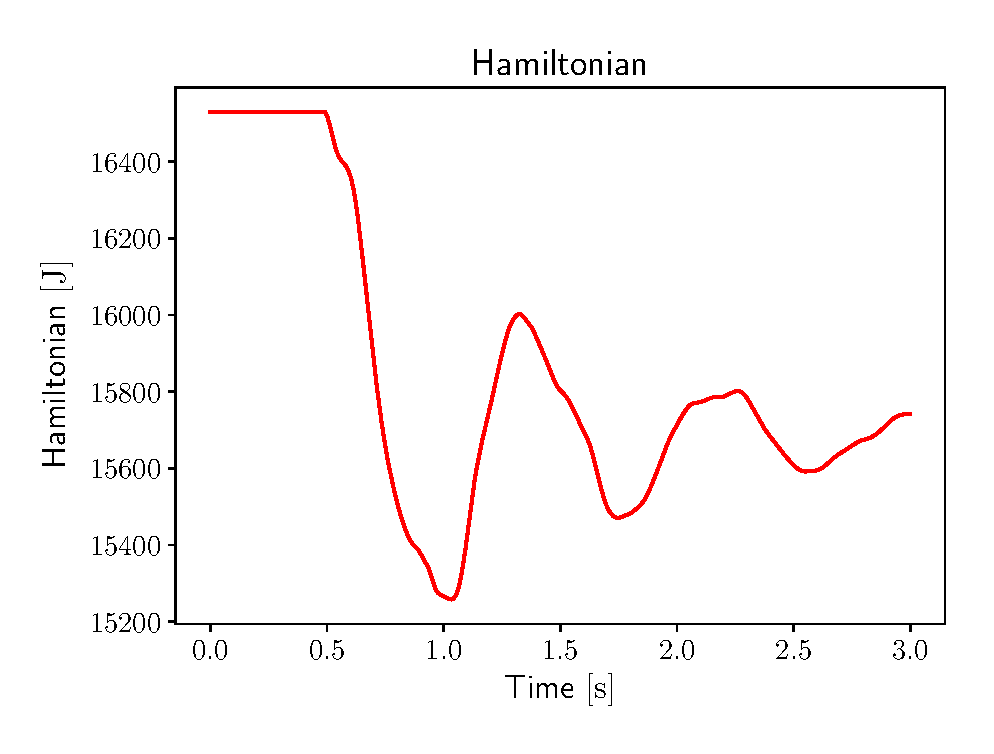
\includegraphics[width=0.48\textwidth]{part_3/applications/bs_SWE/Hamiltonian.eps}
\includegraphics[width=0.48\textwidth]{part_3/applications/bs_SWE/Lyapunov.eps}
\end{center}
}
\end{frame}

\subsection{The linear case}

\begin{frame}
\begin{assumption}[Quadratic separable Hamiltonian]
	The Hamiltonian is assumed to be a positive quadratic separable functional in $\bm{\alpha}_1, \, \bm{\alpha}_2$ 
	\begin{equation*}
	H = \frac{1}{2} \inner[L^2(\Omega, \mathbb{A})]{\bm{\alpha}_{1}}{\mathcal{Q}_1\bm{\alpha}_{1}} + \frac{1}{2} \inner[L^2(\Omega, \mathbb{B})]{\bm{\alpha}_{2}}{\mathcal{Q}_2\bm{\alpha}_{2}},
	\end{equation*}
	where $\mathcal{Q}_1, \, \mathcal{Q}_2$ are positive symmetric operators, bounded from below and above
	\begin{equation*}
	m_1 \bm{I}_\mathbb{A} \le\mathcal{Q}_1 \le M_1 \bm{I}_\mathbb{A}, \qquad  m_2 \bm{I}_\mathbb{B} \le \mathcal{Q}_2 \le M_2 \bm{I}_\mathbb{B}, \qquad m_1>0, \ m_2>0, \ M_1>0, \ M_2>0.
	\end{equation*} 
\end{assumption}


\begin{exampleblock}{PH linear system}
\begin{equation*}
\begin{bmatrix}
\mathcal{M}_1 & 0 \\
0 & \mathcal{M}_2 \\
\end{bmatrix}
\partial_t \begin{pmatrix}
\bm{e}_1 \\ \bm{e}_2
\end{pmatrix} = \begin{bmatrix}
0 &  - \mathcal{L}^* \\
\mathcal{L} & 0 \\
\end{bmatrix}\begin{pmatrix}
\bm{e}_1 \\ \bm{e}_2
\end{pmatrix} , \qquad \begin{aligned}
\bm{e}_1 &\in H^{\mathcal{L}}, 	\\
\bm{e}_2 &\in H^{-\mathcal{L}^*},
\end{aligned}
\end{equation*}
where $\mathcal{M}_1:=\mathcal{Q}_1^{-1},\; \mathcal{M}_2:=\mathcal{Q}_2^{-1}$. \textbf{Constitutive laws} have been included in the dynamics.
\end{exampleblock}

\end{frame}

\begin{frame}{The linear discretized system}
\begin{exampleblock}{Finite dimensional system for $\bm{u}_\partial = \mathcal{N}_{\partial, 1} \displaystyle \bm{e}_1, \;  \bm{y}_\partial = \mathcal{N}_{\partial, 2} \displaystyle \bm{e}_2$}
	\begin{equation*}
	\begin{aligned}
	\begin{bmatrix}
	\mathbf{M}_{\mathcal{M}_1} & \mathbf{0} \\
	\mathbf{0} & \mathbf{M}_{\mathcal{M}_2} \\
	\end{bmatrix}
	\begin{pmatrix}
	\dot{\mathbf{e}}_{1} \\
	\dot{\mathbf{e}}_{2} \\
	\end{pmatrix}
	&= \begin{bmatrix}
	\mathbf{0} & \mathbf{D}_{-\mathcal{L}^*} \\
	- \mathbf{D}_{-\mathcal{L}^*}^\top & \mathbf{0} \\
	\end{bmatrix} 
	\begin{pmatrix}
	\mathbf{e}_{1} \\
	\mathbf{e}_{2} \\
	\end{pmatrix} + 
	\begin{bmatrix}
	\mathbf{0}\\
	\mathbf{B}_2\\
	\end{bmatrix}
	\mathbf{u}_\partial, \\
	\mathbf{M}_\partial {\mathbf{y}_\partial} &= 
	\begin{bmatrix}
	\mathbf{0} & \mathbf{B}_2^\top 
	\end{bmatrix}\begin{pmatrix}
	\mathbf{e}_{1} \\
	\mathbf{e}_{2} \\
	\end{pmatrix}.
	\end{aligned}
	\end{equation*}
\end{exampleblock}

\begin{exampleblock}{Finite dimensional system for $\bm{u}_\partial = \mathcal{N}_{\partial, 2} \displaystyle \bm{e}_2, \; \bm{y}_\partial = \mathcal{N}_{\partial, 1} \displaystyle \bm{e}_1$}
	\begin{equation*}
	\begin{aligned}
	\begin{bmatrix}
	\mathbf{M}_{\mathcal{M}_1} & \mathbf{0} \\
	\mathbf{0} & \mathbf{M}_{\mathcal{M}_2} \\
	\end{bmatrix}
	\begin{pmatrix}
	\dot{\mathbf{e}}_{1} \\
	\dot{\mathbf{e}}_{2} \\
	\end{pmatrix}
	&= \begin{bmatrix}
	\mathbf{0} & - \mathbf{D}_{\mathcal{L}}^\top \\
	\mathbf{D}_{\mathcal{L}} & \mathbf{0} \\
	\end{bmatrix} 
	\begin{pmatrix}
	\mathbf{e}_{1} \\
	\mathbf{e}_{2} \\
	\end{pmatrix} + 
	\begin{bmatrix}
	\mathbf{B}_1\\
	\mathbf{0}\\
	\end{bmatrix}
	\mathbf{u}_\partial, \\
	\mathbf{M}_\partial {\mathbf{y}_\partial} &= \begin{bmatrix}
	\mathbf{B}_1^\top & \mathbf{0}
	\end{bmatrix}\begin{pmatrix}
	\mathbf{e}_{1} \\
	\mathbf{e}_{2} \\
	\end{pmatrix}.
	\end{aligned}
	\end{equation*}
\end{exampleblock}
	
\end{frame}

\begin{frame}{Power balance}
The power balance 
\begin{equation*}
\dot{H}_d = \mathbf{e}_1^\top \mathbf{M}_{\mathcal{M}_1} \dot{\mathbf{e}}_{1} + \mathbf{e}_2^\top \mathbf{M}_{\mathcal{M}_2} \dot{\mathbf{e}}_{2} 
\end{equation*}
mimics the continuous one.

\begin{exampleblock}{Causality $\bm{u}_\partial = \mathcal{N}_{\partial, 1} \displaystyle \bm{e}_1$}
	
	\begin{equation*}
	\begin{aligned}
	\dot{H}_d &= \mathbf{e}_{1}^\top \mathbf{D}_{-\mathcal{L}^*} \mathbf{e}_{2} - \mathbf{e}_{2}^\top \mathbf{D}_{-\mathcal{L}^*}^\top \mathbf{e}_{1} + \mathbf{e}_{2}^\top \mathbf{B}_2 \mathbf{u}_\partial, \\
	& = \mathbf{y}_\partial^\top \mathbf{M}_\partial \mathbf{u}_\partial
	\end{aligned}
	\end{equation*}
	
\end{exampleblock}

\begin{exampleblock}{Causality $\bm{u}_\partial = \mathcal{N}_{\partial, 2} \displaystyle \bm{e}_2$}
	
	\begin{equation*}
	\begin{aligned}
	\dot{H}_d 	&= - \mathbf{e}_{1}^\top \mathbf{D}_{\mathcal{L}}^\top \mathbf{e}_{2} + \mathbf{e}_{2}^\top \mathbf{D}_{\mathcal{L}} \mathbf{e}_{1} + \mathbf{e}_{1}^\top \mathbf{B}_1 \mathbf{u}_\partial, \\
	& = \mathbf{y}_\partial^\top \mathbf{M}_\partial \mathbf{u}_\partial.
	\end{aligned}
	\end{equation*}
	
\end{exampleblock}
\end{frame}


\subsection{Mixed boundary conditions}

\begin{frame}{Mixed boundary conditions (linear system)}

Consider now the following boundary-control linear pH system in co-energy form 
\begin{columns}
\begin{column}{0.6\textwidth}
\begin{align*}
\begin{bmatrix}
\mathcal{M}_1 & 0 \\
0 & \mathcal{M}_2 \\
\end{bmatrix}
\partial_t \begin{pmatrix}
\bm{e}_1 \\ \bm{e}_2
\end{pmatrix} &= \begin{bmatrix}
0 &- \mathcal{L}^* \\
\mathcal{L} & 0 \\
\end{bmatrix}\begin{pmatrix}
\bm{e}_1 \\ \bm{e}_2
\end{pmatrix}, \\
\begin{pmatrix}
\bm{u}_{\partial, 1}\\
\bm{u}_{\partial, 2}\\
\end{pmatrix} &= \begin{bmatrix}
\mathcal{N}_{\partial, 1}^{\Gamma_1} & 0\\
0 & \mathcal{N}_{\partial, 2}^{\Gamma_2} \\
\end{bmatrix} \begin{pmatrix}
\bm{e}_1 \\ \bm{e}_2
\end{pmatrix}, \\
\begin{pmatrix}
\bm{y}_{\partial, 1}\\
\bm{y}_{\partial, 2}\\
\end{pmatrix} &= \begin{bmatrix}
0 & \mathcal{N}_{\partial, 2}^{\Gamma_1} \\
\mathcal{N}_{\partial, 1}^{\Gamma_2} & 0\\
\end{bmatrix} \begin{pmatrix}
\bm{e}_1 \\ \bm{e}_2
\end{pmatrix}.
\end{align*}
\end{column}
\begin{column}{0.4\textwidth}
\begin{figure}[tb]
	\centering
	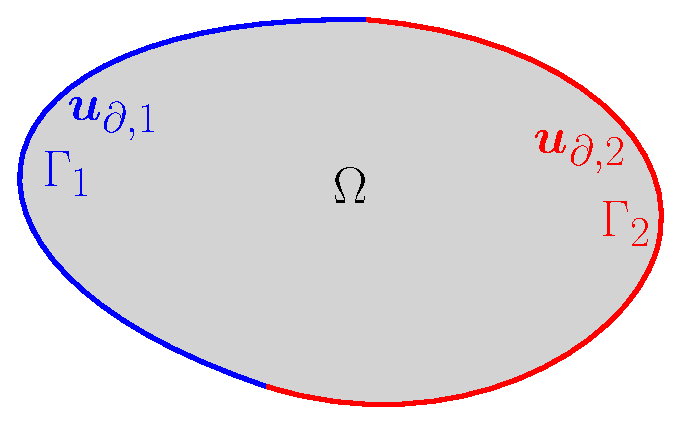
\includegraphics[width=0.9\columnwidth]{part_3/pfem/bound_part.eps}
\end{figure}
\end{column}
\end{columns}

\vspace{1cm}
The operator $\mathcal{N}_{\partial, *}^{\Gamma_\circ}$ with $*, \circ \in \{1, 2\}$ represents now the restriction of operator $\mathcal{N}_{\partial, *}$ over the subset $\Gamma_\circ$.
\end{frame}

\begin{frame}{Lagrange multiplier method}
A Lagrange multiplier can be introduced to include the input that does not explicitly appear in the weak formulation, i.e. to enforce the essential boundary condition. 
\only<1>{
\begin{block}{Integration by parts of $-\mathcal{L}^*$ ($\bm\lambda_{\partial, 1}=\bm{u}_{\partial, 1}$) }
\begin{equation*}
\begin{aligned}
\mathrm{Diag}
\begin{bmatrix}
\mathbf{M}_{\mathcal{M}_1}\\
\mathbf{M}_{\mathcal{M}_2}\\
\mathbf{0}\\
\end{bmatrix}
\begin{pmatrix}
\dot{\mathbf{e}}_{1} \\
\dot{\mathbf{e}}_{2} \\
\dot{\bm{\lambda}}_{\partial, 1} \\
\end{pmatrix}
&= \begin{bmatrix}
\mathbf{0} & - \mathbf{D}_{\mathcal{L}}^\top & \mathbf{B}_{1, \Gamma_1}\\
\mathbf{D}_{\mathcal{L}} & \mathbf{0} & \mathbf{0} \\
-\mathbf{B}_{1, \Gamma_1}^\top & \mathbf{0} & \mathbf{0} \\
\end{bmatrix} 
\begin{pmatrix}
\mathbf{e}_{1} \\
\mathbf{e}_{2} \\
{\bm{\lambda}}_{\partial, 1} \\
\end{pmatrix} + 
\begin{bmatrix}
\mathbf{0} & \mathbf{B}_{1, \Gamma_2} \\
\mathbf{0} & \mathbf{0} \\
\mathbf{M}_{\partial, 1} & \mathbf{0} \\
\end{bmatrix}
\begin{bmatrix}
\mathbf{u}_{\partial, 1} \\
\mathbf{u}_{\partial, 2} \\
\end{bmatrix}, \\
\begin{bmatrix}
\mathbf{M}_{\partial, 1} & \mathbf{0} \\
\mathbf{0} & \mathbf{M}_{\partial, 2} \\
\end{bmatrix}
\begin{pmatrix}
\mathbf{y}_{\partial, 1} \\
\mathbf{y}_{\partial, 2} \\
\end{pmatrix}
&= \begin{bmatrix}
\mathbf{0} & \mathbf{0} & \mathbf{M}_{\partial, 1} \\
\mathbf{B}_{1, \Gamma_2}^\top & \mathbf{0} & \mathbf{0} \\
\end{bmatrix}\begin{pmatrix}
\mathbf{e}_{1} \\
\mathbf{e}_{2} \\
{\bm{\lambda}}_{\partial, 1} \\
\end{pmatrix}.
\end{aligned}
\end{equation*}
\end{block}
}


\only<2>{
\begin{block}{Integration by parts of $\mathcal{L}$ ($\bm{\lambda}_{\partial, 2} = \bm{u}_{\partial, 2}$)}
	\begin{equation*}
	\begin{aligned}
	\mathrm{Diag}
	\begin{bmatrix}
	\mathbf{M}_{\mathcal{M}_1}\\
	\mathbf{M}_{\mathcal{M}_2}\\
	\mathbf{0}\\
	\end{bmatrix}
	\begin{pmatrix}
	\dot{\mathbf{e}}_{1} \\
	\dot{\mathbf{e}}_{2} \\
	\dot{\bm{\lambda}}_{\partial, 2} \\
	\end{pmatrix}
	&= \begin{bmatrix}
	\mathbf{0} & \mathbf{D}_ {-\mathcal{L}^*} & \mathbf{0}\\
	- \mathbf{D}_ {-\mathcal{L}^*}^\top & \mathbf{0} & \mathbf{B}_{2, \Gamma_2} \\
	\mathbf{0} & -\mathbf{B}_{2, \Gamma_2}^\top & \mathbf{0}  \\
	\end{bmatrix} 
	\begin{pmatrix}
	\mathbf{e}_{1} \\
	\mathbf{e}_{2} \\
	{\bm{\lambda}}_{\partial, 2} \\
	\end{pmatrix} + 
	\begin{bmatrix}
	\mathbf{0} & \mathbf{0} \\
	\mathbf{B}_{2, \Gamma_1} & \mathbf{0} \\
	\mathbf{0} & \mathbf{M}_{\partial, 2} \\
	\end{bmatrix}
	\begin{bmatrix}
	\mathbf{u}_{\partial, 1} \\
	\mathbf{u}_{\partial, 2} \\
	\end{bmatrix}, \\
	\begin{bmatrix}
	\mathbf{M}_{\partial, 1} & \mathbf{0} \\
	\mathbf{0} & \mathbf{M}_{\partial, 2} \\
	\end{bmatrix}
	\begin{pmatrix}
	\mathbf{y}_{\partial, 1} \\
	\mathbf{y}_{\partial, 2} \\
	\end{pmatrix}
	&= \begin{bmatrix}
	\mathbf{0} & \mathbf{B}_{2, \Gamma_1}^\top & \mathbf{0} \\
	\mathbf{0} & \mathbf{0} & \mathbf{M}_{\partial, 2} \\
	\end{bmatrix}\begin{pmatrix}
	\mathbf{e}_{1} \\
	\mathbf{e}_{2} \\
	{\bm{\lambda}}_{\partial, 2} \\
	\end{pmatrix}.
	\end{aligned}
	\end{equation*}
\end{block}
}

\end{frame}

\begin{frame}{Power balance}
The energy balance
\begin{equation*}
\dot{H}_d = \mathbf{e}_1^\top \mathbf{M}_{\mathcal{M}_1} \dot{\mathbf{e}}_1 + \mathbf{e}_2^\top \mathbf{M}_{\mathcal{M}_2} \dot{\mathbf{e}}_2
\end{equation*}
mimics the continuous counterpart.
\begin{exampleblock}{Integration by parts of $-\mathcal{L}^*$ ($\bm{\lambda}_{\partial, 1} = \bm{u}_{\partial, 1}$)}
\begin{equation*}
\begin{aligned}
\dot{H}_d &= -\mathbf{e}_1^\top \mathbf{D}_\mathcal{L}^\top {\mathbf{e}}_2 + \mathbf{e}_2^\top\mathbf{D}_\mathcal{L} {\mathbf{e}}_1 + \mathbf{e}_1^\top (\mathbf{B}_{1, \Gamma_1} \bm{\lambda}_{\partial, 1} + \mathbf{B}_{1, \Gamma_2} \mathbf{u}_{\partial, 2} ), \\
&= \mathbf{y}_{\partial, 1}^\top \mathbf{M}_{\partial, 1} \mathbf{u}_{\partial, 1} + \mathbf{y}_{\partial, 2}^\top \mathbf{M}_{\partial, 2} \mathbf{u}_{\partial, 2}. 
\end{aligned}
\end{equation*}
\end{exampleblock}
\begin{exampleblock}{Integration by parts of $\mathcal{L}$ ($\bm{\lambda}_{\partial, 2} = \bm{u}_{\partial, 2}$)}
	\begin{equation*}
	\begin{aligned}
	\dot{H}_d &= \mathbf{e}_1^\top \mathbf{D}_{-\mathcal{L}^*}^\top {\mathbf{e}}_2 - \mathbf{e}_2^\top\mathbf{D}_{-\mathcal{L}^*} {\mathbf{e}}_1 + \mathbf{e}_2^\top (\mathbf{B}_{2, \Gamma_2} \bm{\lambda}_{\partial, 2} + \mathbf{B}_{2, \Gamma_1} \mathbf{u}_{\partial, 1} ), \\
	&= \mathbf{y}_{\partial, 1}^\top \mathbf{M}_{\partial, 1} \mathbf{u}_{\partial, 1} + \mathbf{y}_{\partial, 2}^\top \mathbf{M}_{\partial, 2} \mathbf{u}_{\partial, 2}. 
	\end{aligned}
	\end{equation*}
\end{exampleblock}
\end{frame}

\begin{frame}{Example: cantilever Kirchhoff plate}

\begin{equation*}
\begin{bmatrix}
\rho h & 0 \\ 
\bm{0} & \bm{\mathcal{D}_b}^{-1} \\
\end{bmatrix}
\diffp{}{t}
\begin{pmatrix}
e_w \\ \bm{E}_\kappa \\
\end{pmatrix} = 
\begin{bmatrix}
0 & -\div\Div \\ 
\Grad\grad & \bm{0} \\
\end{bmatrix}
\begin{pmatrix}
e_w \\ \bm{E}_\kappa \\
\end{pmatrix} \qquad (x, y) \in \Omega = [0, 1]\times[0,1],
\end{equation*}
subject to Dirichlet homogeneous conditions and Neumann boundary control
\begin{align*}
\begin{aligned}
\partial_t e_w|_{\Gamma_D} &= 0, \\
\partial_x e_w|_{\Gamma_D} &= 0, \\
\end{aligned} \qquad {\Gamma_D} = \left\{x = 0 \right\}, \qquad
\begin{aligned}
u_{\partial, q} & = \widetilde{q}_n|_{\Gamma_N},\\
u_{\partial, m} &= M_{nn}|_{\Gamma_N}.\\
\end{aligned} \qquad {\Gamma_N} = \left\{y = 0 \cup x=1 \cup y=1 \right\}.
\end{align*}

\begin{columns}
	\begin{column}{.5\textwidth}
		The corresponding boundary outputs read
		\begin{equation*}
		\begin{aligned}
		y_{\partial, q} &= e_w|_{\Gamma_N}, \\
		y_{\partial, m} &=\partial_{\bm{n}} e_w|_{\Gamma_N}.
		\end{aligned}
		\end{equation*}
		
		The following control law stabilizes the system
		\begin{equation*}
		\begin{aligned}
		u_{\partial, q} & = - k y_{\partial, q}, \\
		u_{\partial, m} & = - k y_{\partial, m}, \\
		\end{aligned} \qquad k>0.
		\end{equation*}
		
	\end{column}

	\begin{column}{.5\textwidth}
		\begin{figure}[b]
			\centering
			\includegraphics[width=0.9\columnwidth]{part_3/applications/bs_Kirchh/plate_controlled.eps}
		\end{figure}
	\end{column}
\end{columns}

\end{frame}


\begin{frame}{Discretization strategy}

The $\div\Div$ operator is integrated by parts twice to enforce weekly the Neumann conditions. The \firedrake library is used to generate the matrices. The Dirichlet condition is imposed weakly through a Lagrange multiplier (strong imposition of boundary conditions for $H^2$ conforming elements is not trivial \footfullcite{kirby2019}). 

\begin{table}[t]
	\centering
	\begin{tabular}{|c|c|}
		\hline 
		\multicolumn{2}{|c|}{Plate Parameters} \\ 
		\hline 
		$E$ & $70\; \mathrm{[GPa]}$ \\ 
		$\rho$ & $2700\; \mathrm{[kg \cdot m^3]}$ \\ 
		$\nu$& $0.35$ \\ 
		$h/L$& $0.05$ \\ 
		$L_x = L_y$& $1\; \mathrm{[m]}$\\ 
		\hline 
	\end{tabular} \hspace{.1cm}
	\begin{tabular}{|c|c|}
		\hline 
		\multicolumn{2}{|c|}{Simulation Settings} \\
		\hline 
		Integrator & St\"ormer-Verlet \\
		$\Delta t $ & $1 \; \mathrm{[\mu s]}$ \\  
		N$_{\text{dof}}^\circ$ & $2574$ \\
		FE spaces & ($e_w \approx $ Argyris) $\times$ ($\bm{E}_\kappa \approx$ DG$_3$) $\times$ ($\bm{\lambda} \approx$ CG$_2$)\\
		$t_{\text{end}}$ & $5\; \mathrm{[s]}$\\ 
		\hline 
	\end{tabular} 
\end{table}

	Control parameter 
	\begin{equation*}
	k_* = 
	\begin{cases}
	0, \quad &\forall t < 1 \, [\mathrm{s}], \\
	10, \quad &\forall t \ge 1 \, [\mathrm{s}].
	\end{cases}
	\end{equation*}

	
\end{frame}

\begin{frame}{Results cantilever Kirchoff plate}
\only<1>{
\begin{center}
\includemedia[
label=vidDam,
addresource=/home/a.brugnoli/Videos_defense/Kirchh_Damped_3s.mp4,
activate=pageopen,
width=10cm, height=5cm,
flashvars={
	source=/home/a.brugnoli/Videos_defense/Kirchh_Damped_3s.mp4
	&loop=true
}
]{}{VPlayer.swf}

\mediabutton[
mediacommand=vidDam:playPause,
]{\fbox{Play/Pause}}
\end{center}
}
\only<2>{
\begin{figure}[htb]
	\centering
	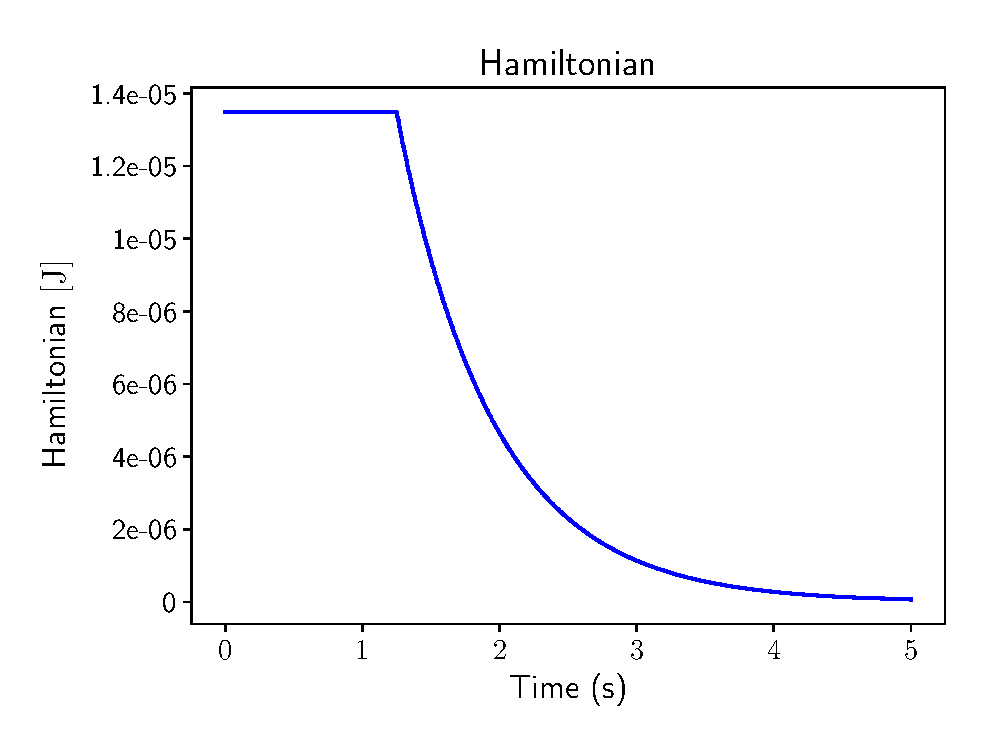
\includegraphics[width=0.7\textwidth]{part_3/applications/bs_Kirchh/Hamiltonian.eps}
\end{figure}
}
%\movie[width=0.42\textwidth, height = 0.7 \textheight]{Damped Kirchhoff Plate}{../Videos/Kirchh_Damped_4faster.mp4}
\end{frame}


\begin{frame}{Virtual domain decomposition}
The idea is based on the fact that a mixed boundary conditions problem can be split into two problems with uniform causality. The two systems are then appropriately interconnected.

\begin{figure}[b]
	\begin{minipage}[b]{0.4\linewidth}
		\centering
		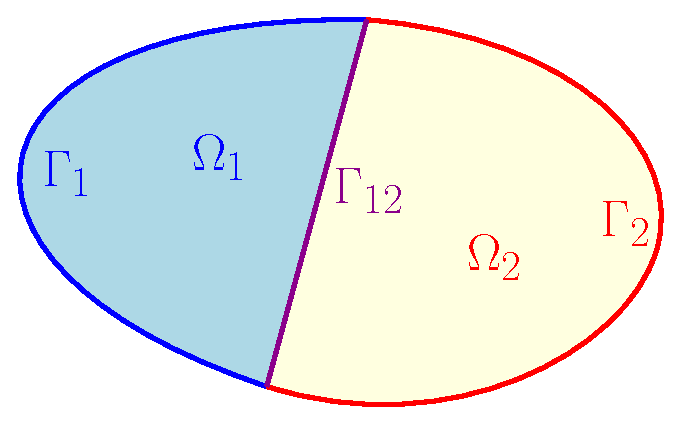
\includegraphics[width=0.95\textwidth]{part_3/pfem/dom_part.eps}
		\caption{Splitting of the domain.}
	\end{minipage}
	\hspace{0.5cm}
	\begin{minipage}[b]{0.55\linewidth}
		\centering
		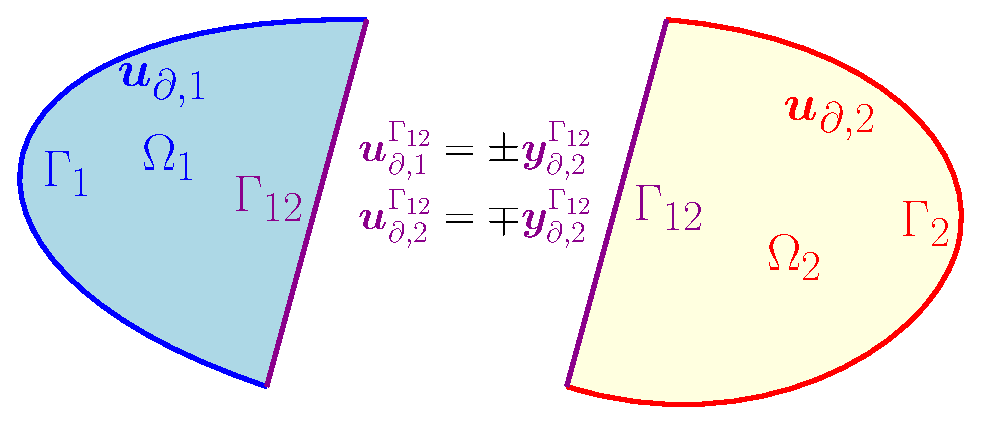
\includegraphics[width=0.95\textwidth]{part_3/pfem/dom_part_int.eps}
		\caption{Interconnection at the interface $\Gamma_{12}$.}
	\end{minipage}
\end{figure}

\end{frame}

\begin{comment}
\begin{frame}{Core idea}
For $\Omega_1$ subdomain, we set

\begin{equation*} 
\begin{pmatrix}
\bm{u}_{\partial, 1}\\
\textcolor{blue}{\bm{u}_{\partial, 1}^{\Gamma_{12}}}\\
\end{pmatrix} = \begin{bmatrix}
\mathcal{N}_{\partial, 1}^{\Gamma_1} & 0\\
\mathcal{N}_{\partial, 1}^{\Gamma_{12}} & 0 \\
\end{bmatrix} \begin{pmatrix}
\bm{e}_1 \\ \bm{e}_2
\end{pmatrix}, \qquad
\begin{pmatrix}
\bm{y}_{\partial, 1}\\
\textcolor{red}{\bm{y}_{\partial, 1}^{\Gamma_{12}}} \\
\end{pmatrix} = \begin{bmatrix}
0 & \mathcal{N}_{\partial, 2}^{\Gamma_1} \\
0 & \mathcal{N}_{\partial, 2}^{\Gamma_{12}} \\
\end{bmatrix} \begin{pmatrix}
\bm{e}_1 \\ \bm{e}_2
\end{pmatrix},
\end{equation*}
whereas for the $\Omega_2$ subdomain
\begin{equation*}
\begin{pmatrix}
\bm{u}_{\partial, 2}\\
\textcolor{red}{\bm{u}_{\partial, 2}^{\Gamma_{12}}}\\
\end{pmatrix} = \begin{bmatrix}
0 & \mathcal{N}_{\partial, 2}^{\Gamma_2}\\
0 & \mathcal{N}_{\partial, 2}^{\Gamma_{12}} \\
\end{bmatrix} \begin{pmatrix}
\bm{e}_1 \\ \bm{e}_2
\end{pmatrix}, \qquad
\begin{pmatrix}
\bm{y}_{\partial, 2}\\
\textcolor{blue}{\bm{y}_{\partial, 2}^{\Gamma_{12}}}\\
\end{pmatrix} = \begin{bmatrix}
\mathcal{N}_{\partial, 1}^{\Gamma_1} & 0 \\
\mathcal{N}_{\partial, 1}^{\Gamma_{12}}  & 0 \\
\end{bmatrix} \begin{pmatrix}
\bm{e}_1 \\ \bm{e}_2
\end{pmatrix}.
\end{equation*}
The following relations then hold
\begin{equation*}
\textcolor{blue}{\bm{u}_{\partial, 1}^{\Gamma_{12}}} =\pm \textcolor{blue}{\bm{y}_{\partial, 2}^{\Gamma_{12}}}, \qquad \textcolor{red}{\bm{u}_{\partial, 2}^{\Gamma_{12}}} = \mp \textcolor{red}{\bm{y}_{\partial, 1}^{\Gamma_{12}}}.
\end{equation*}
The plus or minus sign is due to the fact that either $\mathcal{N}_{\partial, 1}^{\Gamma_{12}}$ or $\mathcal{N}_{\partial, 2}^{\Gamma_{12}}$ contains a scalar product with the outgoing normal (or the tangent unit vector) at ${\Gamma_{12}}$ (that has opposite direction depending on which subdomain is considered).
\end{frame}
\end{comment}


\begin{frame}{Summary: mixed boundary conditions}

\begin{tcbraster}[raster columns=2, raster equal height]
	\begin{tcolorbox}[width=0.4\textwidth, nobeforeafter, colframe=theme,title=Lagrange multiplier]%%
		\begin{itemize}
			\item[\textcolor{green}{\checkmark}] Easier implementation (only one mesh);
			\item[\textcolor{red}{$\times$}] Must fulfill the \textit{inf-sup} condition;	
			\item[\textcolor{red}{$\times$}] Requires solving a DAE, or specific reduction methods.
		\end{itemize}
	\end{tcolorbox} 
	\begin{tcolorbox}[width=0.4\textwidth, nobeforeafter,  colframe=theme,title=Virtual domain decomposition]%%
		\begin{itemize}
			\item[\textcolor{green}{\checkmark}] Provides an ODE;
			\item[\textcolor{red}{$\times$}] Requires the construction of multiple meshes;
			\item[\textcolor{red}{$\times$}] Different formulation (and therefore finite elements) on each subdomain;
		\end{itemize}
	\end{tcolorbox}
\end{tcbraster}
\end{frame}

\subsection{Convergence study: the Mindlin plate example}


\begin{frame}{The Mindlin plate under clamped boundary conditions}

\begin{equation*}
	\begin{bmatrix}
	\rho b  & 0  & 0  & 0 \\
	\bm{0} & I_\theta &  \bm{0} & \bm{0}\\
	\bm{0}  & \bm{0}  & \bm{\mathcal{C}}_b  & \bm{0}\\
	\bm{0} & \bm{0} &  \bm{0} & C_s \\
	\end{bmatrix}
	\diffp{}{t}
	\begin{pmatrix}
	e_w \\
	\bm{e}_\theta \\
	\bm{E}_\kappa \\
	\bm{e}_{\gamma} \\
	\end{pmatrix} = 
	\begin{bmatrix}
	0  & 0  & 0  & \div \\
	\bm{0} & \bm{0} &  \Div & \bm{I}_{2 \times 2}\\
	\bm{0}  & \Grad  & \bm{0}  & \bm{0}\\
	\grad & -\bm{I}_{2 \times 2} &  \bm{0} & \bm{0} \\
	\end{bmatrix}
	\begin{pmatrix}
	e_w \\
	\bm{e}_{\theta} \\
	\bm{E}_{\kappa} \\
	\bm{e}_{\gamma} \\
	\end{pmatrix} + 
	\begin{pmatrix}
	f \\
	\bm{\tau} \\
	\bm{0} \\
	\bm{0} \\
	\end{pmatrix}, \qquad
	\begin{aligned}
	{e}_w\vert_{\partial\Omega} &= 0, \\
	\bm{e}_\theta\vert_{\partial\Omega} &= \bm{0}.
	\end{aligned}	
\end{equation*}
where $b$ is the thickness, $I_\theta$ is the rotary inertia, $\bm{C}_b, \; C_s$ are the bending and shear compliance  respectively, $f, \; \bm{\tau}$ are distributed forces and torques.
\vspace{.5cm}

For this example, the $\mathcal{L}, \; -\mathcal{L}^*, \; \mathcal{N}_{\partial, 1}, \; \mathcal{N}_{\partial, 2}$ operators are given by
\begin{equation*}
\mathcal{L} = \begin{bmatrix}
\bm{0} & \Grad\\
\grad & -\bm{I}_{2 \times 2}\\
\end{bmatrix}, \quad
-\mathcal{L}^* = \begin{bmatrix}
\bm{0} & \div\\
\Div & \bm{I}_{2 \times 2}\\
\end{bmatrix}, \qquad
\mathcal{N}_{\partial, 1} = \begin{bmatrix}
\gamma_0 & 0 \\ 
0 &  \bm\gamma_0\\
\end{bmatrix}, \quad 
\mathcal{N}_{\partial, 2} = \begin{bmatrix}
0 & \gamma_{n}  \\
\bm\gamma_n & 0 \\
\end{bmatrix}.
\end{equation*}

\end{frame}

\begin{frame}{Mixed discretization}
\setlength{\abovedisplayskip}{3pt}
\setlength{\belowdisplayskip}{3pt}
After integrating by parts $\mathcal{L}$, the weak form looks for solutions in the space
$$\{e_w, \bm{e}_{\bm{\theta}}, \bm{E}_{\kappa}, \bm{e}_{\gamma}\} \in L^2(\Omega) \times L^2(\Omega, \bbR^2) \times H^{\Div}(\Omega, \bbR^{2\times 2}_{\text{sym}}) \times H^{\div}(\Omega, \bbR^2).$$
The clamped condition is a natural one in this setting.
\begin{block}{BJT elements}
These elements were proposed in Bécache 2001 for elastodynamics problems\footfullcite{becache2001elas}.
\begin{figure}
\centering
\includegraphics[width=0.8\textwidth]{presentation/fe_BJT.eps}
\end{figure}
		
\end{block}

\end{frame}



\begin{frame}{Dual mixed formulation}
\setlength{\abovedisplayskip}{3pt}
\setlength{\belowdisplayskip}{3pt}
If instead $-\mathcal{L}^*$ the weak form looks for solutions in the space
$$\{e_w, \bm{e}_{\bm{\theta}}, \bm{E}_{\kappa}, \bm{e}_{\gamma}\} \in H^{1}(\Omega) \times H^{\Grad}(\Omega, \bbR^2) \times L^2(\Omega, \bbR^{2\times 2}_{\text{sym}}) \times L^2(\Omega, \bbR^2).$$
The clamped condition is an essential one in this setting.
\begin{block}{CG elements}
Conforming elements for a similar problem are detailed in Cohen 2007\footfullcite{cohen2007mindlin}.
\begin{figure}
	\centering
	\includegraphics[width=0.8\textwidth]{presentation/fe_CG.eps}
\end{figure}
		
\end{block}

\end{frame}


\begin{frame}{Conjectured convergence estimates}

\begin{conjecture}[Convergence rate for the BJT elements]
	\setlength{\abovedisplayskip}{0pt}
	\setlength{\belowdisplayskip}{0pt}
	Combining previous results \footfullcite{becache2000wave,becache2001elas}, the following error estimates can be conjectured. Assuming a smooth solution, the following error estimates hold 
	\begin{equation*}
	\label{eq:errBEC}
	\begin{aligned}
	||e_w - e_w^h||_{L^{\infty}(L^2(\Omega))} &\lesssim h^{k}, \\
	||\bm{e}_\theta - \bm{e}_\theta^h||_{L^{\infty}(L^2(\Omega, \bbR^2))} &\lesssim h^{k}, \\
	\end{aligned} \qquad
	\begin{aligned}
	||\bm{E}_\kappa - \bm{E}_\kappa^h||_{L^{\infty}(L^2(\Omega, \bbR^{2\times 2}_{\text{sym}}))} &\lesssim  h^{k}, \\
	||\bm{e}_\gamma - \bm{e}_\gamma^ h||_{L^{\infty}(L^2(\Omega, \bbR^2))} &\lesssim  h^{k}. \\
	\end{aligned} 
	\end{equation*}
\end{conjecture}

\begin{conjecture}[Convergence of the CG elements]
\setlength{\abovedisplayskip}{0pt}
\setlength{\belowdisplayskip}{0pt}
	Assuming a smooth solution, the following error estimates hold 
	\begin{equation*}
	\label{eq:errCGDG}
	\begin{aligned}
	||e_w - e_w^h||_{L^{\infty}(H^1(\Omega))} &\lesssim h^{k}, \\
	||\bm{e}_\theta - \bm{e}_\theta^h||_{L^{\infty}(H^{\Grad}(\Omega, \bbR^2))} &\lesssim h^{k}, \\
	\end{aligned} \qquad
	\begin{aligned}
	||\bm{E}_\kappa - \bm{E}_\kappa^h||_{L^{\infty}(L^2(\Omega, \bbR^{2\times 2}_{\text{sym}}))} &\lesssim  h^{k}, \\
	||\bm{e}_\gamma - \bm{e}_\gamma^ h||_{L^{\infty}(L^2(\Omega, \bbR^2))} &\lesssim  h^{k}. \\
	\end{aligned} 
	\end{equation*}
	
\end{conjecture}
\end{frame}

\begin{comment}

\begin{frame}{An analytical solution for the clamped Mindlin plate}
\setlength{\abovedisplayskip}{4pt}
\setlength{\belowdisplayskip}{4pt}
\onslide<1->{

A static solution is already known for this problem defined on the unit square domain\footfullcite{veiga2013}:
\begin{equation*}
\begin{aligned}
0 &= \mathrm{div} \ \bm{q}_s + f_s , \\
0 &= \mathrm{Div} \bm{M}_s + \bm{q}_s, \\
\end{aligned} \qquad
\begin{aligned}
\bm{\mathcal{C}}_b\bm{M}_s &= \mathrm{Grad} \ \bm{\theta}_s, \\
C_s \bm{q}_s &= \mathrm{grad} \ w_s - \bm{\theta}_s, \\
\end{aligned}
\qquad
\begin{aligned}
w_s\vert_{\partial\Omega} = 0, \\
\bm{\theta}_s\vert_{\partial\Omega} = 0. \\
\end{aligned}
\end{equation*}
}

\onslide<2->{
A solution for the dynamic problem is obtained considering
\[
w_d(x,y,t) = w_s(x,y) \sin(t), \quad \bm{\theta}_d(x,y,t) = \bm\theta_s(x,y) \sin(t).
\]
}
\onslide<3->{
Appropriate forcing terms have to be introduced to compensate the inertial accelerations
\begin{equation*}
f_d = f_s \sin(t) + \rho b \partial_{tt} w_d, \qquad \bm{\tau}_d = \frac{\rho b^3}{12} \partial_{tt} \bm{\theta}_d.
\end{equation*}
}
\onslide<4>{
The exact solution and boundary conditions for the pH system are thus given by
\begin{equation*}
\begin{aligned}
e_w^\text{ex} &= w_s(x,y) \cos(t), \\
\bm{e}_\theta^\text{ex} &= \bm\theta_s(x,y) \cos(t), \\
\end{aligned} \qquad
\begin{aligned}
\bm{E}_\kappa^\text{ex} &=  \bm{\mathcal{D}}_b \ \mathrm{Grad} \ \bm{\theta}_d, \\
\bm{e}_\gamma^\text{ex} &= D_s(\mathrm{grad} \ w_d - \bm{\theta}_d), \\
\end{aligned}
\qquad
\begin{aligned}
e_w^\text{ex}\vert_{\partial\Omega} &= 0, \\
\bm{e}_\theta^\text{ex}\vert_{\partial\Omega} &= 0. \\
\end{aligned}
\end{equation*}
}

\end{frame}
\end{comment}

\begin{frame}{Simulation Settings}
\begin{itemize}
	\item The {\sc{Firedrake}} library is used to generate the matrices. 
	\item Time integration: a Crank-Nicholson scheme has been used with time step $\Delta t = h/10$ where $h$ is the mesh size.
	\item Linear solver: Conjugate gradient with LU preconditioner.
	\item To compute the $L^\infty ({X})$ space-time dependent norm  the discrete norm $L^\infty_{\Delta t} ({X})$ is used
	\[
	||\cdot ||_{L^\infty ({X})} \approx || \cdot ||_{L^\infty_{\Delta t} ({X})} = \max_{t \in t_i} ||\cdot||_{{X}},
	\]
	where $t_i$ are the discrete simulation instants.
\end{itemize}

 \begin{table}[htbp]
 	\centering
 	\begin{tabular}{ccccc}
 		\hline 
 		\multicolumn{5}{c}{Plate parameters} \\ 
 		\hline 
 		$E$ & $\rho$ & $\nu$ & $K_{\text{sh}}$ & $b$ \\
 		$74 \;  [\textrm{GPa}]$ & $2700\; [\textrm{kg}/\textrm{m}^3]$ & $0.3$ & $5/6$ &  $0.1 \;  [\textrm{m}]$\\ 
 		\hline 
 	\end{tabular} 
 	\caption{Physical parameters for the Numerical test (Aluminum).}
 \end{table}
\end{frame}

\begin{frame}{Results}
\only<1>{
	\begin{figure}[b]
		\begin{minipage}[b]{0.45\linewidth}
			\centering
			\includegraphics[width=1\textwidth]{presentation/CCCC_BEC_Phys_vel.eps}
			\caption{BTJ $e_w$ error ($L^\infty(L^2(\Omega))$).}
		\end{minipage}
		\begin{minipage}[b]{0.45\linewidth}
			\centering
			\includegraphics[width=1\textwidth]{presentation/CCCC_CF_Phys_vel.eps}
			\caption{CG $e_w$ error ($L^\infty(H^1(\Omega))$).}
		\end{minipage}
	\end{figure}
}
\only<2>{
	\begin{figure}[b]
		\begin{minipage}[b]{0.45\linewidth}
			\centering
			\includegraphics[width=1\textwidth]{presentation/CCCC_BEC_Phys_om.eps}
			\caption{BTJ $\bm{e}_\theta$ error ($L^\infty(L^2(\Omega, \bbR^2))$).}
		\end{minipage}
		\begin{minipage}[b]{0.45\linewidth}
			\centering
			\includegraphics[width=1\textwidth]{presentation/CCCC_CF_Phys_om.eps}
			\caption{CG $\bm{e}_\theta$ error ($L^\infty(H^{\Grad}(\Omega, \bbR^2))$).}
		\end{minipage}
	\end{figure}
}
\only<3>{
	\begin{figure}[b]
		\begin{minipage}[b]{0.45\linewidth}
			\centering
			\includegraphics[width=1\textwidth]{presentation/CCCC_BEC_Phys_sig.eps}
			\caption{BTJ $\bm{E}_\kappa$ error ($L^\infty(L^2(\Omega, \bbR^{2\times 2}_{\text{sym}}))$).}
		\end{minipage}
		\begin{minipage}[b]{0.45\linewidth}
			\centering
			\includegraphics[width=1\textwidth]{presentation/CCCC_CF_Phys_sig.eps}
			\caption{CG $\bm{E}_\kappa$ error ($L^\infty(L^2(\Omega, \bbR^{2\times 2}_{\text{sym}}))$).}
		\end{minipage}
	\end{figure}
}
\only<4>{
	\begin{figure}[b]
		\begin{minipage}[b]{0.45\linewidth}
			\centering
			\includegraphics[width=1\textwidth]{presentation/CCCC_BEC_Phys_q.eps}
			\caption{BTJ $\bm{e}_\gamma$ error ($L^\infty(L^2(\Omega, \bbR^{2}))$).}
		\end{minipage}
		\begin{minipage}[b]{0.45\linewidth}
			\centering
			\includegraphics[width=1\textwidth]{presentation/CCCC_CF_Phys_q.eps}
			\caption{CG $\bm{e}_\gamma$ error ($L^\infty(L^2(\Omega, \bbR^{2}))$).}
		\end{minipage}
	\end{figure}
}
\end{frame}

\section{PH flexible multibody dynamics}

\begin{frame}{Previous work}

Using Lie Algebra and differential forms a pH model of a flexible link has already been proposed \footfullcite{macchelli2007link}. This model can be embedded in a complex multibody system\footfullcite{macchelli2009multi}. \\

\begin{overlayarea}{\textwidth}{0.55\textheight}
	\setlength{\abovedisplayskip}{1pt}
	\setlength{\belowdisplayskip}{1pt}
	Advantages:
	\begin{itemize}
		\item {Modular construction of flexible systems;}
		\item {Large deformations naturally considered.}
	\end{itemize}
	Drawbacks:
	\begin{itemize}
		\item {Quite cumbersome implementation;}
		\item {Limited to one-dimensional beam;}
		\item {Numerical analysis not feasible;}
		\item {Model reduction techniques not easily applicable.} 
	\end{itemize}
\end{overlayarea}
\end{frame}

\begin{frame}{Floating frame based approach}
The floating frame approach relies on the hypothesis of small deformations: elastic motion is described w.r.t a reference that follows the large rigid motion\footfullcite{wasfy2003survey}. \\
\begin{overlayarea}{\textwidth}{0.5\textheight}
	Advantages 
	\begin{itemize}
		\item {The most used paradigm in multibody dynamics;}
		\item {For control applications other approaches are too complex;}
		\item {Linear model reduction techniques are applicable.} 
	\end{itemize}
	Drawbacks:
	\begin{itemize}
		\item {Effect due to geometric non-linearities are not considered: not suitable for large deformations (substructuring can be employed to alleviate this).}
	\end{itemize}
\end{overlayarea}
\end{frame}

\begin{frame}{Floating body kinematics}
\onslide*<1>{
	\begin{tcolorbox}
		\begin{figure}[t]
			\centering
			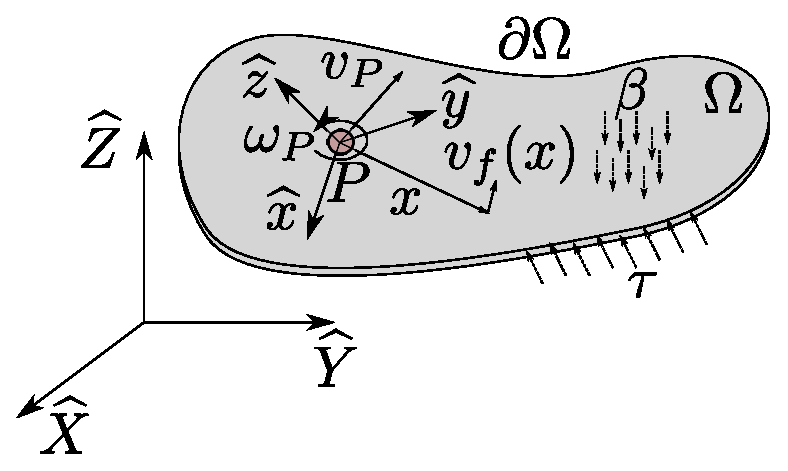
\includegraphics[width=0.6\textwidth]{part_4/pHfmd/floating_body.eps} 
			\caption{Thin floating body undergoing a surface traction $\bm\tau$ and body force density $\bm\beta$}
			\label{fig:float_body}
		\end{figure}
	\end{tcolorbox}
}
\onslide*<2->{
	The velocity of a generic point is expressed by considering a small flexible displacement superimposed to the rigid motion
	\[
	\bm{v} = \bm{v}_P + \crmat{\bm{\omega}_P} (\bm{x}+\bm{u}_f) + \bm{v}_f.
	\]
	where the cross map $\crmat{\bm{a}}$ denotes the skew-symmetric matrix associated to vector $\bm{a}$. \\
	
	This equation is expressed in the body reference frame $\widehat{\bm{x}}, \widehat{\bm{y}}, \widehat{\bm{z}}$. 
	
}
\onslide<3->{
\vspace{5pt}
Kinematic variables:  
\begin{itemize}
	\item $\bm{x}$ is the position vector of the current point;
	\item $\bm{v}_P,\, \bm{\omega}_P$ are the linear and angular velocities of point $P$;
	\item $\bm{v}_f := \dot{\bm{u}}_f$ the deformation velocity.
\end{itemize}
}
\onslide<4>{
Inertia terms:
\begin{itemize}
	\item $m:= \int_{\Omega} \rho \d{\Omega}$ the total mass;
	\item $\bm{s}_u:= \int_{\Omega} \rho (\bm{x}+\bm{u}_f) \d{\Omega}$ the static moment;
	\item $\bm{J}_u:= \int_{\Omega} \rho \crmat{\bm{x}+\bm{u}_f}^\top\crmat{\bm{x}+\bm{u}_f} \d{\Omega}$ the inertia matrix.
\end{itemize}
	
}
\end{frame}

\subsection{PH formulation of a floating body}

\begin{frame}{Canonical momenta}
\begin{overlayarea}{\textwidth}{0.95\textheight}
	Consider the total energy (Hamiltonian), given by the sum of kinetic and deformation energy:
	\begin{equation*}
	H = H_{\text{kin}} + H_{\text{def}}= \frac{1}{2} \int_{\Omega} \left\{\rho ||\bm{v}_P + \crmat{\bm{\omega}_P} (\bm{x}+\bm{u}_f) + {\bm{v}}_f||^2 + \bm\Sigma \cddot \bm\varepsilon \right\}  \d{\Omega}.
	\end{equation*}
	
	\only<1>{ 
		\begin{exampleblock}{Canonical momenta}
			\begin{equation*}
			\begin{aligned}
			\bm{p}_t &:= \diffp{H}{\bm{v}_P} = m \bm{v}_P + \crmat{\bm{s}_u}^\top \, \bm\omega_P + \int_{\Omega} \rho \bm{v}_f \d{\Omega}, \\
			\bm{p}_r &:= \diffp{H}{\bm\omega_P} = \crmat{\bm{s}_u} \bm{v}_P + \bm{J}_u \bm\omega_P + \int_{\Omega} \rho \crmat{\bm{x}+\bm{u}_f} \bm{v}_f \d{\Omega}, \\
			\bm{p}_f &:= \diffd{H}{\bm{v}_f} = \rho \bm{v}_P + \rho \crmat{\bm{x}+\bm{u}_f}^\top \, \bm\omega_P + \rho \bm{v}_f, \\
			\bm\varepsilon &:= \diffd{H}{\bm\Sigma} = \bm{\mathcal{D}}^{-1} \bm\Sigma,
			\end{aligned}
			\end{equation*}
		\end{exampleblock} 
		
	}
	\only<2>{
		\begin{exampleblock}{Canonical momenta}
			\setlength{\abovedisplayskip}{1pt}
			\setlength{\belowdisplayskip}{1pt}
			\begin{equation*}
			\begin{bmatrix}
			\bm{p}_t \\ \bm{p}_r \\ \bm{p}_f \\ \bm\varepsilon \\
			\end{bmatrix} = 
			\underbrace{\begin{bmatrix}
				m \bm{I}_{3\times 3} & \crmat{\bm{s}_u}^\top & \mathcal{I}_\rho^{\Omega} & 0 \\
				\crmat{\bm{s}_u} & \bm{J}_u & \bm{\mathcal{I}}_{\rho x}^{\Omega} & 0  \\
				(\mathcal{I}_\rho^{\Omega})^* & (\bm{\mathcal{I}}_{\rho x}^{\Omega})^* & \rho & 0  \\
				0 & 0 & 0 & \bm{\mathcal{D}}^{-1} \\
				\end{bmatrix}}_{\mathcal{M}: \; \text{Mass operator}}
			\begin{bmatrix}
			\bm{v}_P \\ \bm{\omega}_P  \\ \bm{v}_f  \\ \bm\Sigma \\
			\end{bmatrix}, \qquad 
			\begin{aligned}
			\mathcal{I}_\rho^\Omega &:=\int_{\Omega} \rho (\cdot) \d{\Omega}, \\
			\bm{\mathcal{I}}_{\rho x}^{\Omega} &:= \int_\Omega \rho \crmat{\bm{x}+\bm{u}_f} (\cdot). \\
			\end{aligned}
			\end{equation*}	
			The mass operator $\mathcal{M}$ is a self-adjoint, positive operator. It holds
			\begin{equation*}
			H_{\text{kin}} + H_{\text{def}} = \frac{1}{2} \langle \bm{e}_{\text{kd}}, \ \mathcal{M} \bm{e}_{\text{kd}} \rangle, \qquad \bm{e}_{\text{kd}} = [\bm{v}_P; \, \bm{\omega}_P; \, \bm{v}_f; \bm{\Sigma}]
			\end{equation*}
		\end{exampleblock} 
	}
	
	\only<3>{
	\begin{exampleblock}{Modified canonical momenta}
	\setlength{\abovedisplayskip}{1pt}
	\setlength{\belowdisplayskip}{1pt}
	\begin{equation*}
	\begin{aligned}
	\widehat{\bm{p}}_t &:=  m \bm{v}_P + \crmat{\bm{s}_u}^\top \, \bm\omega_P + 2\int_{\Omega} \rho \bm{v}_f \d{\Omega}, \\
	\widehat{\bm{p}}_r &:=  \crmat{\bm{s}_u} \bm{v}_P + \bm{J}_u \bm\omega_P + 2 \int_{\Omega} \rho \crmat{\bm{x}+\bm{u}_f} \bm{v}_f \d{\Omega}, \\
	\end{aligned} \qquad 
	\begin{aligned}
	\widehat{\bm{p}}_f &:= \rho \bm{v}_P + \rho \crmat{\bm{x}+\bm{u}_f}^\top \, \bm\omega_P + 2\rho \bm{v}_f, \\
	\bm{\mathcal{I}}_{p_f}^\Omega &:= \int_\Omega \left\{ \crmat{\bm{p}_f} + \crmat{\widehat{\bm{p}}_f} \right\}(\cdot) \d{\Omega},
	\end{aligned} 
	\end{equation*}
	\end{exampleblock} 
	Notice that the kinetic energy also depends on the flexible displacement
	\[
	\diffd{H_{\text{kin}}}{\bm{u}_f} = \crmat{\bm{p}_f} \bm{\omega}_{P}.
	\]
	}
\end{overlayarea}
\end{frame}



\begin{frame}{Generalized coordinates}
Generalized coordinates are required for a complete formulation:
\begin{itemize}
	\item $^i \bm{r}_P$ the position of point $P$ in the inertial frame of reference;
	\item $\bm{R}$ the direction cosine matrix (other attitude parametrizations are possible);
	\item $\bm{u}_f$ the flexible displacement;
\end{itemize}
The direction cosine matrix is converted into a vector by concatenating its rows
\begin{equation*}
\bm{R}_{\text{v}} = \text{vec}(\bm{R}^\top) = [\bm{R}_1 \; \bm{R}_2 \; \bm{R}_3]^\top,
\end{equation*}
where $\bm{R}_{1}, \bm{R}_{2}, \bm{R}_{3}$ are the rows of matrix $\bm{R}$. Furthermore the corresponding cross map will be given by
\begin{equation*}
\crmat{\bm{R}_{\text{v}}} = 
\begin{bmatrix}
\crmat{\bm{R}_1} \\
\crmat{\bm{R}_2} \\
\crmat{\bm{R}_3} \\
\end{bmatrix}, \qquad 
\crmat{\bm{R}_{\text{v}}} : \mathbb{R}^9 \rightarrow \mathbb{R}^{9 \times 3}.
\end{equation*}
\end{frame}

\begin{frame}{PH formulation}
The overall port-Hamiltonian formulation (without including the boundary traction $\bm{\tau}$)
\begin{equation*}
\setlength{\dashlinegap}{2pt}
\underbrace{
{\left[ \begin{array}{c:c}
	\bm{I} & 0 \\
	\hdashline
	0 & \mathcal{M} \\
	\end{array} \right]}
}_{\mathcal{E}}
\diffp{}{t}
\underbrace{\begin{bmatrix}
^i \bm{r}_P \\ \bm{R}_{\text{v}} \\ \bm{u}_f \\\hdashline  \bm{v}_P \\ \bm\omega_P  \\ \bm{v}_f  \\ \bm\Sigma \\
\end{bmatrix}}_{\bm{e}} = 
\underbrace{
{\left[ \begin{array}{ccc:cccc}
	0 & 0 & 0 &  \bm{R} & 0 & 0 & 0 \\
	0 & 0 & 0 & 0 & \crmat{\bm{R}_{\text{v}}} & 0 & 0 \\
	0 & 0 & 0 & 0 & 0 & \bm{I}_{3\times 3} & 0  \\ 
	\hdashline
	-\bm{R}^\top & 0 & 0 & 0 & \crmat{\widehat{\bm{p}}_t} & 0 & 0 \\
	0 & -\crmat{\bm{R}_{\text{v}}}^\top & 0 & \crmat{\widehat{\bm{p}}_t} & \crmat{\widehat{\bm{p}}_r} & \bm{\mathcal{I}}_{p_f}^\Omega & 0 \\
	0 & 0 & -\bm{I}_{3\times 3} & 0 & -(\bm{\mathcal{I}}_{p_f}^\Omega)^* & 0 & \Div \\
	0 & 0 & 0 & 0 & 0 & \Grad & 0 \\
	\end{array} \right]}
}_{\mathcal{J}}
\underbrace{\begin{bmatrix}
\partial_{\bm{r}_P}H \\ \partial_{\bm{R}_\text{v}}H \\ \delta_{\bm{u}_f} H \\\hdashline  \bm{v}_P \\ \bm\omega_P  \\ \bm{v}_f  \\ \bm\Sigma \\
\end{bmatrix}}_{\bm{z}}.
\end{equation*} 

\end{frame}

\begin{frame}{Floating body as a pHDAE system}
\begin{exampleblock}{Final pHDAE system}
	This system fits into the framework detailed in Morandin 2019 \footfullcite{mehrmann2019structurepreserving} and extends it.
	\begin{equation*}
	\begin{aligned}
	\mathcal{E}(\bm{e}) \partial_t \bm{e} &= \mathcal{J}(\bm{e}) \bm{z}(\bm{e}) + {\mathcal{B}}_r(\bm{e}) \bm{u}_\partial, \\
	\bm{y}_r &= {\mathcal{B}}_r^*(\bm{e}) \bm{z}(\bm{e}), \\
	\bm{u}_\partial &= {\mathcal{B}}_{\partial} \bm{z}(\bm{e}) =  \bm\Sigma \cdot \bm{n}|_{\partial \Omega} = \bm\tau|_{\partial \Omega}, \\
	\bm{y}_\partial &= {\mathcal{C}}_{\partial} \bm{z}(\bm{e}) = \bm{v}_f|_{\partial \Omega},
	\end{aligned}
	\end{equation*}
	with $\bm{y}_r = (\bm{v}_P + \crmat{\bm{x}+\bm{u}_f}^\top \bm{\omega}_P)\vert_{\partial\Omega}$.
\end{exampleblock}
Operator ${\mathcal{E}}$ is positive self-adjoint, ${\mathcal{J}}$ is formally skew-symmetric.
The Hamiltonian  satisfies 
\begin{equation*}
\partial_{\bm{e}} H = {\mathcal{E}}^* \bm{z}.
\end{equation*}
\end{frame}

\begin{frame}{Energy balance}

\begin{exampleblock}{Power balance}
	The power balance equals the power due to the surface traction
	\begin{equation*}
	\setlength{\abovedisplayskip}{5pt}
	\setlength{\belowdisplayskip}{5pt}
	\begin{aligned}
	\dot{H}(\bm{e}) &= \langle \partial_{\bm{e}} H, \partial_t {\bm{e}} \rangle_{X},\\
	&= \langle \bm{z}, {\mathcal{E}} \partial_t {\bm{e}} \rangle_{{X}}, \quad \text{Adjoint definition},  \\
	&= \langle \bm{y}_\partial,  \bm{u}_\partial \rangle_{\partial\Omega} + \langle {\mathcal{B}}_r^* \bm{z}, \bm{u}_\partial \rangle_{\partial\Omega}, \quad \text{I.B.P. on } {\mathcal{J}}, \\
	&=  \int_{\partial \Omega} \bm{u}_\partial \cdot (\bm{y}_\partial + \bm{y}_r)  \d{\Omega}, \\
	&= \int_{\partial \Omega} \bm\tau \cdot \bm{v} \d\Gamma,  \\
	\end{aligned}
	\end{equation*}
	where $\bm{y}_\partial + \bm{y}_r := (\bm{v}_P + \crmat{\bm{\omega}_P} (\bm{x}+\bm{u}_f) + {\bm{v}}_f)\vert_{\partial\Omega} = \bm{v}\vert_{\partial\Omega}$ is the velocity field at the boundary.
\end{exampleblock}

\end{frame}

\begin{frame}{Some remarks}

\begin{itemize}
	\item Generic linear elastic model can be included (beams, plates etc.).
	\item Conservative forces are easily accounted for by introducing an appropriate potential energy. For example, the gravitational potential reads
	\begin{equation*}
	H_{\text{pot}} = \int_{\Omega} \rho g \, ^i r_z \d{\Omega} = \int_{\Omega} \rho g \left[ ^i r_{P, z} +\bm{R}_z (\bm{x} + \bm{u}_f) \right] \d{\Omega}.
	\end{equation*}
	\item If case of vanishing deformations $\bm{u}_f \equiv 0$, the Newton-Euler equations on the Euclidean group $SE(3)$ are retrieved
	\begin{equation*}
	\diff{}{t}
	\begin{pmatrix}
	^i{\bm{r}}_P \\
	\bm{R}_{\mathrm{v}} \\
	{\bm{p}}_t \\ 
	{\bm{p}}_r \\
	\end{pmatrix} = 
	\begin{bmatrix}
	0 & 0 & \bm{R} & 0 \\
	0 & 0 & 0 & \crmat{\bm{R}_{\text{v}}} \\
	- \bm{R}^\top & 0 & 0 & \crmat{\bm{p}_t}\\
	0 & -\crmat{\bm{R}_{\text{v}}}^\top & \crmat{\bm{p}_t} & \crmat{\bm{p}_r} \\
	\end{bmatrix}
	\begin{bmatrix}
	\partial_{\bm{r}_P} H \\ 
	\partial_{\bm{R}_{\text{v}}} H \\ 
	\partial_{\bm{p}_t} H \\ 
	\partial_{\bm{p}_r} H \\ 
	\end{bmatrix}.
	\end{equation*}
\end{itemize}
\end{frame}

\subsection{Discretization}

\begin{frame}{Discretized system}
Same procedure as always but the integration by parts is applied to the $\Div$ operator to highlight the Neumann condition.
\begin{exampleblock}{Finite-dimensional pHDAE system}
	\setlength{\abovedisplayskip}{3pt}
	\setlength{\belowdisplayskip}{3pt}
	After integration by parts of the $\Div$ operator
	\begin{equation*}
	\begin{aligned}
	\mathbf{E}(\mathbf{e}) \dot{\mathbf{e}} &= \mathbf{J}(\mathbf{e}) \mathbf{z}(\mathbf{e}) + \mathbf{B}_\partial(\mathbf{e}) \mathbf{u}_\partial, \\
	\mathbf{M}_\partial \mathbf{y}_\partial &= \mathbf{B}_\partial^\top \mathbf{z}(\mathbf{e}).
	\end{aligned}
	\end{equation*}
\end{exampleblock}

\begin{block}{Dirichlet conditions}
	The set $\Gamma_D$ for the Dirichlet condition has to be non empty, otherwise the deformation field is allowed for rigid movement, leading to a singular mass matrix: test and state shape functions must verify a homogeneous Dirichlet condition\footfullcite{agrawal1986application}. 
\end{block}
\end{frame}

\subsection{Example: boundary interconnection of the Kirchhoff plate}

\begin{frame}{Rigid rod welded to a cantilever plate }
\begin{tcolorbox}
	\centering
	\only<1>{ 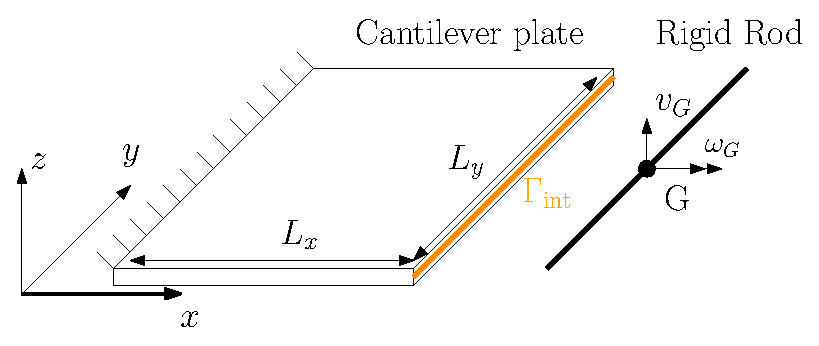
\includegraphics[width=0.9\textwidth]{part_4/validation/KP/plate_rod_separated.eps}}
	\only<2>{\includegraphics[width=0.7\textwidth]{part_4/validation/KP/plate_rod_welded.eps}}
\end{tcolorbox}

\end{frame}


\begin{frame}{Boundary Interconnection}
\centering \includegraphics[width=0.6\textwidth]{part_4/validation/KP/pp_interconnection.eps}
\end{frame}


\begin{frame}{Results}
\begin{center}
\onslide*<1>{
\setlength{\abovedisplayskip}{0pt}
\setlength{\belowdisplayskip}{0pt}
\begin{equation*}
\text{Load} \qquad f = \begin{cases}
10^5 \left[ y + 10 \left( y - L_y/2 \right)^2 \right] [\mathrm{Pa}], \quad &\forall \, t < 2 \, [\mathrm{ms}], \\
0, \quad &\forall \, t \ge 2 \, [\mathrm{ms}],
\end{cases}
\quad t_{\text{end}} = 10 \, [\mathrm{ms}].
\end{equation*}
\begin{columns}
\begin{column}{.45\textwidth}
	\includemedia[
	label=vidNoRod,
	addresource=/home/a.brugnoli/Videos_defense/Kirchh_NoRod.mp4,
	activate=pageopen,
	width=6cm, height=5cm,
	flashvars={
		source=/home/a.brugnoli/Videos_defense/Kirchh_NoRod.mp4
		&loop=true
	}
	]{}{VPlayer.swf}
\end{column}
\begin{column}{.45\textwidth}
	\includemedia[
	label=vidRod,
	addresource=/home/a.brugnoli/Videos_defense/Kirchh_Rod.mp4,
	activate=pageopen,
	width=6cm, height=5cm,
	flashvars={
		source=/home/a.brugnoli/Videos_defense/Kirchh_Rod.mp4
		&loop=true
	}
	]{}{VPlayer.swf}
\end{column}
\end{columns}

\mediabutton[
mediacommand=vidNoRod:playPause,
mediacommand=vidRod:playPause
]{\fbox{Play/Pause}}

%\movie[width=0.8\textwidth, height=0.6\textheight]{Plate and rod}{../Videos/Comparison_RodNoRod.mp4}	
}

\onslide*<2>{
\includegraphics[width=0.48\textwidth]{part_4/validation/KP/HamiltonianNoRod.eps}
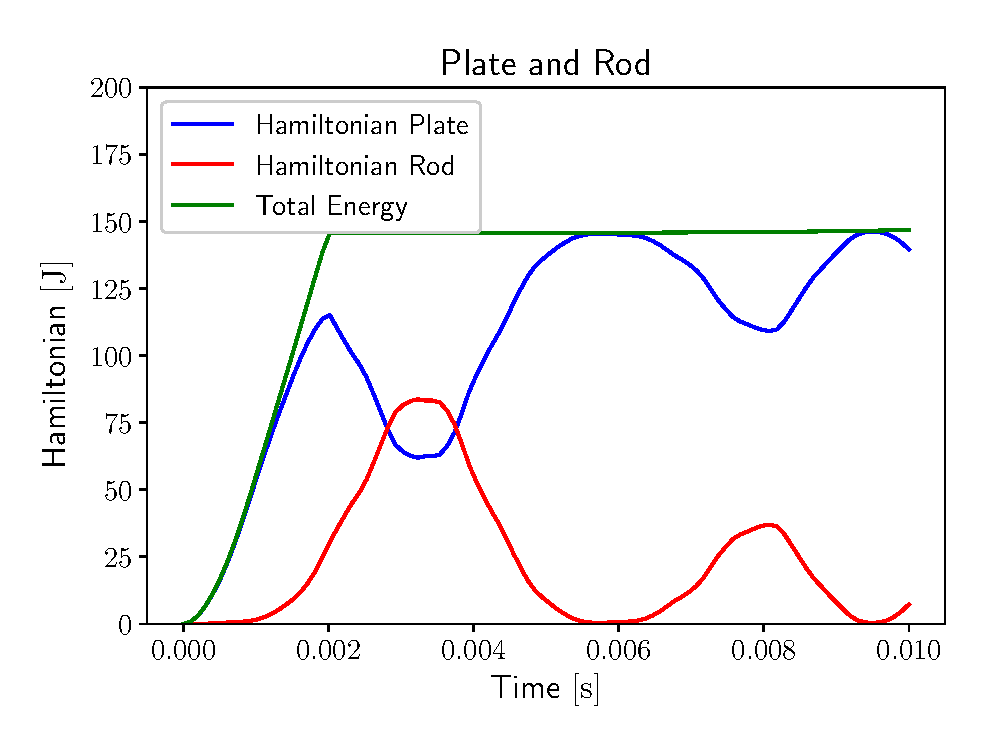
\includegraphics[width=0.48\textwidth]{part_4/validation/KP/HamiltonianRod.eps}
}

\end{center}
\end{frame}



\begin{frame}{Conclusion}
Main contributions:
\begin{itemize}
\item \onslide<2->{A port-Hamiltonian formulation of elasticity, thermoelasticity and plate problems;}
\item \onslide<3->{Development and validation of a finite element based symplectic discretization characterized by an easy re-implementability;}
\item \onslide<4->{Floating frame based multibody dynamics: this multibody framework allows including the linear elastic models discussed in this thesis.}
\end{itemize}

\end{frame}

\begin{frame}{Outlook}
Open problems and possible developments:
\begin{itemize}
	\item \onslide<2->{Modelling: shell problems and non linear elasticity (ex. von Karman plate);}
	\item \onslide<3->{Discretization: efficient finite element for the Kirchhoff plate based on div-div conforming elements \footfullcite{chen2020divDiv};}
	\item \onslide<4->{Model reduction: application of POD methods, $H_2$-optimal strategies or Krilov subspace methods to the considered models;}
	\item \onslide<5->{Multibody dynamics: computational aspect of the general quasi-linear problem (symplectic time-integration);}
	\item \onslide<6>{Control: observer based strategies for boundary control\footfullcite{toledo2020} and reduced LQG design for distributed control\footfullcite{wu2020reduced}.}
\end{itemize}
\end{frame}


\begin{frame}{Journal articles}
\begin{enumerate}
\item \fullcite{brugnoli2019ammmin} 
\vspace{.3cm}
\item \fullcite{brugnoli2019ammkir} 
\vspace{.3cm}
\item \fullcite{brugnoli2020msd} 
\vspace{.3cm}
\item \fullcite{brugnoli2020numerical}
\end{enumerate}
\end{frame}

\begin{frame}{International conferences with proceedings}
\begin{enumerate}
\item \fullcite{brugnoli2019cpde} 
\vspace{.1cm}
\item \fullcite{brugnoli2019cdc} 
\vspace{.1cm}
\item \fullcite{cardoso2019cdc} 
\vspace{.1cm}
\item \fullcite{brugnoli2020wc} 
\vspace{.1cm}
\item \fullcite{brugnoli2020mtns}
\end{enumerate}
\end{frame}

\appendix

\begin{frame}
\end{frame}

\begin{frame}
\end{frame}

\section{Thermoelasticity}

\subsection{General 3D thermoelasticity as coupled pH systems}

\begin{frame}{The heat equation as a pHDAE}
\begin{overlayarea}{\textwidth}{\textheight}
Consider the heat equation
\begin{equation*}\label{eq:heatEq}
\rho c_\epsilon \partial_t T = k \Delta T + r_Q, \qquad \quad \bm{x} \in \Omega \subset \mathbb{R}^d,
\end{equation*}
\only<1>{
\begin{itemize}
\item $c_\epsilon$ the specific heat density at constant strain;
\item $k$ the thermal diffusivity;
\item $r_Q$ an heat source.
\end{itemize}
}
\only<2>{
Given the Hamiltonian
\begin{equation*}
H_T = \frac{1}{2} \int_\Omega \rho c_\epsilon T_0 \left(\frac{T-T_0}{T_0} \right)^2 \d\Omega,
\end{equation*}
the energy variable and corresponding co-energy are
\begin{equation*}
\alpha_T := \rho c_\epsilon (T-T_0), \qquad e_T := \delta_{\alpha_T} {H_T} ={(T-T_0)}/{T_0}.
\end{equation*}
Introducing the heat flux $\bm{j}_Q := -k \grad T$ as algebraic variable
\begin{equation*}
\begin{aligned}
\begin{bmatrix}
1 & 0 \\
\bm{0} & \bm{0} \\
\end{bmatrix}
\diffp{}{t}
\begin{pmatrix}
\alpha_T \\
\bm{j}_Q \\
\end{pmatrix} &= 
\begin{bmatrix}
0 & -\div \\
-\grad & -(T_0 k)^{-1} \\
\end{bmatrix}
\begin{pmatrix}
e_T \\
\bm{j}_Q \\
\end{pmatrix} + 
\begin{bmatrix}
1 \\
\bm{0} \\
\end{bmatrix} u_T, \\
y_T &= \begin{bmatrix}
1 & \bm{0} \\
\end{bmatrix} \begin{pmatrix}
e_T \\
\bm{j}_Q \\
\end{pmatrix}.
\end{aligned}
\end{equation*}
}
\end{overlayarea}

\end{frame}

\begin{frame}{Classical thermoelasticity as two interconnected systems}
Consider again the equation of elasticity with a distributed input $\bm{u}_E$ (a distributed force)
\begin{equation*}
\begin{aligned}
\diffp{}{t}
\begin{pmatrix}
\bm{\alpha}_v \\
\bm{A}_{\varepsilon} \\
\end{pmatrix} &= 
\begin{bmatrix}
\bm{0} & \Div \\
\Grad & \bm{0} \\
\end{bmatrix}
\begin{pmatrix}
\bm{e}_v \\
\bm{E}_{\varepsilon} \\
\end{pmatrix} + 
\begin{bmatrix}
\bm{I}_{d\times d} \\
\bm{0} \\
\end{bmatrix}\bm{u}_E, \\
\bm{y}_E &= \begin{bmatrix}
\bm{I}_{d\times d} & \bm{0} \\
\end{bmatrix}
\begin{pmatrix}
\bm{e}_v \\
\bm{E}_{\varepsilon}
\end{pmatrix},
\end{aligned}
\end{equation*}
and the heat equation
\begin{equation*}
\begin{aligned}
\begin{bmatrix}
1 & 0 \\
\bm{0} & \bm{0} \\
\end{bmatrix}
\diffp{}{t}
\begin{pmatrix}
\alpha_T \\
\bm{j}_Q \\
\end{pmatrix} &= 
\begin{bmatrix}
0 & -\div \\
-\grad & -(T_0 k)^{-1} \\
\end{bmatrix}
\begin{pmatrix}
e_T \\
\bm{j}_Q \\
\end{pmatrix} + 
\begin{bmatrix}
1 \\
\bm{0} \\
\end{bmatrix} u_T, \\
y_T &= \begin{bmatrix}
1 & \bm{0} \\
\end{bmatrix} \begin{pmatrix}
e_T \\
\bm{j}_Q \\
\end{pmatrix},
\end{aligned}
\end{equation*} 

\end{frame}

\begin{frame}{The interconnection}
Consider the  interconnection
\begin{equation*}
\bm{u}_E = - \Div(\bm{\mathcal{C}}_\beta \, y_T), \qquad
u_T = - \bm{\mathcal{C}}_\beta \cddot\Grad(\bm{y}_E). 
\end{equation*}
The interconnection is power preserving since
\begin{equation*}
\bm{u}_E = \mathcal{A}_\beta(y_T), \qquad u_T = - \mathcal{A}_\beta^*(\bm{y}_E), \where  \mathcal{A}_\beta(\cdot) = - \Div(\bm{\mathcal{C}}_\beta \, \cdot).
\end{equation*}
\begin{block}{PH thermoelasticity}
The coupled thermoelastic problem can now be written as
\begin{equation*}
\begin{bmatrix}
\bm{1} & \bm{0} & \bm{0} & \bm{0}\\
\bm{0} & \bm{1} & \bm{0} & \bm{0}\\
0 & 0 & 1 & 0\\
\bm{0} & \bm{0} & \bm{0} & \bm{0}\\
\end{bmatrix}
\diffp{}{t}
\begin{pmatrix}
\bm{\alpha}_v \\
\bm{A}_\varepsilon \\
{\alpha}_T \\
\bm{j}_Q \\
\end{pmatrix} = 
\begin{bmatrix}
\bm{0} & \Div & \mathcal{A}_\beta & \bm{0}\\
\Grad & \bm{0} & \bm{0} & \bm{0} \\
- \mathcal{A}_\beta^* & 0 & 0 & -\div \\
\bm{0} & \bm{0} & -\grad & - (T_0 k)^{-1} \\
\end{bmatrix}
\begin{pmatrix}
\bm{e}_v \\
\bm{E}_\varepsilon \\
{e}_T \\
\bm{j}_Q \\
\end{pmatrix},
\end{equation*}
with total energy given by $H=H_E + H_T$.
\end{block}

\end{frame}

\subsection{Example: the Danilovskaya problem}

\begin{frame}{The classical problem}
The Danilovskaya problem is a one-dimensional thermoelastic model in the infinite half-space $x\ge 0$. We recall the system of equations for the thermoelastic problem in 1D:

\begin{equation*}
\begin{aligned}
\displaystyle \rho \partial_{tt} u &= \partial_x ({\sigma}_{ET}), \qquad x\ge 0,  \\
\displaystyle \rho c_\epsilon \partial_{t} T &= -\partial_x(j_Q) - {C}_\beta \partial_t \varepsilon, \where {C}_\beta:=T_0 \beta(2\mu + 3\lambda),\\
{\sigma}_{ET} &= {\sigma}_E + {\sigma}_{T}, \\
{\sigma}_E &= (2\mu + \lambda) \varepsilon , \\
{\sigma}_T &= - {C}_\beta \theta,  \\
{\varepsilon} &= \partial_x u, \\
{j}_Q &= -k \, \partial_x T.
\end{aligned}
\end{equation*}
the following boundary conditions apply
\begin{equation*}
\begin{aligned}
T(0, t) = T_1 H(t), \\
\lim_{x \rightarrow \infty} T(x, t) = 0, \\
\end{aligned} \qquad 
\begin{aligned}
\sigma_{ET}(0, t) = 0, \\
\lim_{x \rightarrow \infty} u(x, t) = 0, \\
\end{aligned}
\end{equation*}
where $H(t)$ is the Heaviside function.
\end{frame}

\begin{frame}{PH formulation}
A dimensionless constant $c_\delta$ is usually introduced to strengthen the coupling from the mechanical to the thermal domain 
\begin{equation*}
c_\delta = \delta \frac{\rho c_\epsilon (2 \mu + \lambda)}{\beta^2 (3 \lambda + 2 \mu)^2 T_0},
\end{equation*}
where $\delta \in \{0, 1\}$ is a variable for switching on and off the strong coupling. \\
 The problem can now be recast as a pH system in co-energy variables
\begin{equation*}
\begin{bmatrix}
{\rho} & {0} & {0} & {0}\\
{0} & (2\mu + \lambda)^{-1} & {0} & {0}\\
0 & 0 & \rho c_\epsilon T_0 & 0\\
{0} & {0} & {0} & {0}\\
\end{bmatrix}
\diffp{}{t}
\begin{pmatrix}
{e}_v \\
{e}_\varepsilon \\
{e}_T \\
{j}_Q \\
\end{pmatrix} = 
\begin{bmatrix}
{0} & \partial_x & \mathcal{A}_\beta & {0}\\
\partial_x & {0} & {0} & {0} \\
- c_\delta \mathcal{A}_\beta^* & 0 & 0 & -\partial_x \\
{0} & {0} & -\partial_x & - (T_0 k)^{-1} \\
\end{bmatrix}
\begin{pmatrix}
{e}_v \\
{e}_\varepsilon \\
{e}_T \\
\bm{j}_Q \\
\end{pmatrix},
\end{equation*}
where $\mathcal{A}_\beta(\cdot):=-\partial_x({C}_\beta \, \cdot)$, and boundary conditions
\begin{equation*}
\begin{aligned}
e_T(0, t) &= (T_1 - T_0)/T_0 \; H(t), \\
(e_\varepsilon - {C}_\beta e_v)(L, t) &= 0,
\end{aligned}  \qquad 
\begin{aligned}
(e_\varepsilon - {C}_\beta e_v)(0, t) &= 0, \\
j_Q(L, t) &= 0.
\end{aligned}
\end{equation*}
\end{frame}

\begin{frame}{Discretization}
One possible strategy consists in integrating by parts the whole first line and the $\partial_x$ operator in the third line.
\begin{equation*}
\begin{bmatrix}
\mathbf{M}_{\rho} & \mathbf{0} & \mathbf{0} & \mathbf{0}\\
\mathbf{0} & \mathbf{M}_{(2\mu + \lambda)^{-1}} & \mathbf{0} & \mathbf{0} \\
\mathbf{0} & \mathbf{0} & \mathbf{M}_{\rho c_\epsilon T_0} & \mathbf{0} \\
\mathbf{0} & \mathbf{0} & \mathbf{0} & \mathbf{0} \\
\end{bmatrix}
\begin{pmatrix}
\dot{\mathbf{e}}_v\\
\dot{\mathbf{e}}_\varepsilon\\
\dot{\mathbf{e}}_T\\
\dot{\mathbf{e}}_Q\\
\end{pmatrix}
= \begin{bmatrix}
\mathbf{0} & -\mathbf{D}_{\grad}^\top & \mathbf{A}_{\beta} & \mathbf{0}\\
\mathbf{D}_{\grad} & \mathbf{0} & \mathbf{0} & \mathbf{0} \\
-c_\delta \mathbf{A}_{\beta}^\top & \mathbf{0} &  \mathbf{0} & \mathbf{D}_{\grad}^\top \\
\mathbf{0} & \mathbf{0} & -\mathbf{D}_{\grad} & -\mathbf{R}_Q \\
\end{bmatrix}
\begin{pmatrix}
{\mathbf{e}}_v\\
{\mathbf{e}}_\varepsilon\\
{\mathbf{e}}_T\\
{\mathbf{e}}_Q\\
\end{pmatrix}.
\end{equation*}
The coupling matrix $\mathbf{A}_{\beta}$ arises from the discretization of the coupling operator $\mathcal{A}_\beta^*$ where $\mathbf{R}_Q$ represent a dissipation matrix. \\
For this discretization the boundary condition 
\begin{equation*}
e_T(0, t) = \frac{T_1 - T_0}{T_0} H(t), 
\end{equation*}
is imposed strongly as an essential condition.
\end{frame}

\begin{frame}{Settings and parameters}

\only<1>{
The constant $C_x, C_v$ are the characteristic length and velocity of the problem and $\widehat{L}, \; \widehat{t}_{\text{end}}$ are the dimensionless length and time of the problem. 
\begin{table}[htb]
	\centering
	\begin{tabular}{|c|c|}
		\hline 
		\multicolumn{2}{|c|}{Physical Parameters} \\
		\hline 	
		$\lambda$ & $0.85\ 10^9 \; [\mathrm{kg/(cm\cdot s^2)}]$ \\ 
		$\mu$ & $0.56\ 10^9 \; [\mathrm{kg/(cm\cdot s^2)}]$ \\
		$\rho$ & $7.82\ 10^{-3} \; [\mathrm{kg}/\textrm{cm}^3]$ \\ 
		$c_\epsilon$ & $4.61\ 10^6 \; [\mathrm{cm^2/(K\cdot s^2)}]$ \\
		$k$ & $1.7\ 10^3 \; [\mathrm{kg \cdot cm/ (K\cdot s^3)}]$ \\ 
		$\beta$ & $9.03\ 10^{-6} \; [\mathrm{K}^{-1}]$ \\ 
		$T_0$ & $300 \; [\mathrm{K}]$ \\ 
		$L$ & $C_x \ \widehat{L}$ \\
		$C_x$ & ${k}/{(\rho c_\epsilon C_v)}$ \\
		$\widehat{L}$ & $10$ \\
		\hline 
	\end{tabular} \hspace{.5cm}
	\begin{tabular}{|c|c|}
		\hline 
		\multicolumn{2}{|c|}{Simulation Settings} \\ 
		\hline 
		Integrator & Crank-Nicholson\\
		$t_{\text{end}}$& ${C_v}/{C_x} \; \widehat{t}_{\text{end}}$ \\ 
		$C_v$ & $\sqrt{(\lambda + 2 \mu) / \rho}$ \\
		$\widehat{t}_{\text{end}}$ & $4$ \\
		$\Delta t$ & $10^{-3} \ t_{\text{end}}$ \\
		FE spaces& CG$_1$ $\times$ DG$_0$ $\times$ CG$_1$ $\times$ DG$_0$ \\
		N$^\circ$ FE & 200 \\
		\hline 
	\end{tabular} 
	
\end{table}
}

\only<2>{
 The dimensionless displacement field $\widehat{u}$ and temperature $\theta$ are introduced
$$\widehat{u} = \frac{(\lambda + 2\mu)}{C_x {C}_\beta} u,  \qquad \widehat{T} = \frac{T-T_0}{T_0}.$$
The solution in the Laplace domain for the dimensionless variable is given by
\begin{equation*}
\begin{aligned}
\widehat{T}(s) &= \frac{1}{s(C_1^2 - C_2^2)}[(C_1^2- s^2)\exp(-C_1 \widehat{x}) - (C_2^2 - s^2)\exp(-C_2 \widehat{x})], \\
\widehat{u}(s) &= -\frac{1}{s(C_1^2 - C_2^2)}[C_1\exp(-C_1 \widehat{x}) - C_2\exp(-C_2 \widehat{x})], \\
\end{aligned}
\end{equation*}
where $\widehat{x} = x/C_x$ is the dimensionless space variable and $C_1, \; C_2$ are given by
\begin{equation*}
C_1/2(s) = \left[\frac{s}{2} [(1+\delta+s)\pm[(1+\delta+s)^2-4s]^{\frac{1}{2}} ]\right]^{\frac{1}{2}}.
\end{equation*}

}
\end{frame}

\begin{frame}{Numerical results}
\only<1>{
\begin{figure}[p]
	\begin{minipage}[t]{0.48\linewidth}
		\centering
		\includegraphics[width=1\textwidth]{part_3/applications/thermoelasticity/disp_at1_1D.eps} \\
		\caption{Dimensionless displacement ($\widehat{x} = 1$).}
		\label{fig:disp_at1}
	\end{minipage}
	\begin{minipage}[t]{0.48\linewidth}
		\centering
		\includegraphics[width=1\textwidth]{part_3/applications/thermoelasticity/temp_at1_1D.eps}
		\caption{Dimensionless temperature ($\widehat{x} = 1$).}
		\label{fig:temp_at1}
	\end{minipage}
\end{figure}
}
\only<2>{
\begin{figure}%
	\centering
	\subfloat[][$\delta = 0$]{%
		\label{fig:u_delta0}%
		\includegraphics[width=0.48\columnwidth]{part_3/applications/thermoelasticity/plot_u0.eps}}%
	\hspace{8pt}%
	\subfloat[][$\delta = 1$]{%
		\label{fig:u_delta1}%
		\includegraphics[width=0.48\columnwidth]{part_3/applications/thermoelasticity/plot_u1.eps}} \\
	\caption[]{Displacement solution for the Danilovskaya problem.}%
	\label{fig:u_therElas}%
\end{figure}
}
\only<3>{
\begin{figure}
	\centering
	\subfloat[][$\delta = 0$]{%
		\label{fig:theta_delta0}%
		\includegraphics[width=0.48\columnwidth]{part_3/applications/thermoelasticity/plot_T0.eps}}%
	\hspace{8pt}%
	\subfloat[][$\delta = 1$]{%
		\label{fig:theta_delta1}%
		\includegraphics[width=0.48\columnwidth]{part_3/applications/thermoelasticity/plot_T1.eps}} \\
	\caption[]{Temperature solution for the Danilovskaya problem.}%
	\label{fig:theta_therElas}%
\end{figure}
}
\end{frame}

\section{Vibroacoustic under mixed boundary conditions}

\subsection{Model description}

\begin{frame}{General 3D model}
\begin{overlayarea}{\textwidth}{\textheight}
	Model for the propagation of sound in air
	\begin{equation*}
	\diffp{}{t}
	\begin{bmatrix}
	\chi_s p \\
	\mu_0 \bm{v} \\
	\end{bmatrix} = -
	\begin{bmatrix}
	0 & \mathrm{div} \\
	\mathrm{grad} & 0 \\
	\end{bmatrix}
	\begin{bmatrix}
	p \\
	\bm{v} \\
	\end{bmatrix}, \qquad \text{on } \Omega = \{x \in [0, L],\; r \in [0, R],\; \theta = [0, 2 \pi)\}.
	\end{equation*}
	\only<1>{
		\begin{itemize}
			\item $p \in \mathbb{R}$  and $\bm{v} \in \mathbb{R}^3$: variations of pressure and velocity from a steady state;
			\item $\mu_0$: the steady state mass density;
			\item $\chi_s$: adiabatic compressibility factor;
			\item $x, r, \theta$: axial, radial and tangential coordinates.
		\end{itemize}
	}
	\only<2>{
		\begin{columns}[T]
			\setlength{\abovedisplayskip}{3pt}
			\setlength{\belowdisplayskip}{3pt}
			\begin{column}{.45\textwidth}
				Boundary conditions
				\begin{align*}
				p(x, R, \theta) &= - \mathcal{Z}(x, t) \, v_r(x, R, \theta), \\
				\bm{v} \cdot \bm{n}(0, r, \theta) &= -v_x(0, r, \theta) = - f(r), \\
				\bm{v} \cdot \bm{n}(L, r, \theta) &= +v_x(L, r, \theta) = + f(r), 
				\end{align*}
			\end{column}
			\begin{column}{.45\textwidth}
				Initial conditions
				\begin{equation*}
				\begin{aligned}
				p^0(x, r, \theta) &= 0, \\
				v_x^0(x, r, \theta) &= f(r), 
				\end{aligned}  \qquad
				\begin{aligned}
				v_r^0(x, r, \theta) &= g(r), \\
				v_\theta^0(x, r, \theta) &= 0.
				\end{aligned}    
				\end{equation*}
			\end{column}
		\end{columns}
		\vspace{5pt}
		The impedance $\mathcal{Z}$ and the axial $f(r)$ and radial flow $g(r)$ expressions are the following
		\begin{equation*}
		\begin{aligned}
		\mathcal{Z}(x, t) = \mathds{1}\left\{ \frac{1}{3} L \leq \ x \ \leq \frac{2}{3} L, \,  t \geq 0.2 \ t_{\text{fin}} \right\} \mu_0 \, c_0, \\
		f(r) = \left( 1 - \frac{r^2}{R^2} \right) v_0, \qquad
		g(r) = 16 \frac{r^2}{R^4} \left( R - r \right)^2 v_0. 
		\end{aligned}
		\end{equation*}
	}
	\only<3>{
		\centering
		\vspace{2cm}
		\includegraphics[width=0.8\textwidth]{part_3/applications/mixed_bd_waves/bc_3D_sketch.eps}	
	}
\end{overlayarea}
\end{frame}



\begin{frame}{Model reduction by symmetry}
\begin{overlayarea}{\textwidth}{\textheight}

Because of symmetry the model can be reduced to a 2D problem 
\begin{equation*}
\diffp{}{t}
\begin{bmatrix}
\chi_s p \\
\mu_0 v_x \\
\mu_0 v_r \\
\end{bmatrix} = -
\begin{bmatrix}
0 & \partial_x & \partial_r + 1/r \\
\partial_x & 0 & 0 \\
\partial_r & 0 & 0 \\
\end{bmatrix}
\begin{bmatrix}
p \\
v_x \\
v_r \\
\end{bmatrix}, \quad \text{on } \Omega_{\text{r}} = \{x \in [0, L], r \in [0, R]\}.
\end{equation*}
\only<2>{
	The boundary conditions must now account for the symmetry condition at $r=0$
	\begin{align*}
	p(x, R, \theta) &= - \mathcal{Z}(x, t) \, v_r(x, R, \theta), \\
	\bm{v} \cdot \bm{n}(0, r, \theta) &= -v_x(0, r, \theta) = - f(r), \\
	\bm{v} \cdot \bm{n}(L, r, \theta) &= +v_x(L, r, \theta) = + f(r), \\
	\bm{v}\cdot \bm{n}(x, 0) &= v_r(x, 0) =0
	\end{align*}	
}
\only<3>{
	\centering
	\includegraphics[width=0.7\textwidth]{part_3/applications/mixed_bd_waves/bc_2D_sketch.eps}	
}
\end{overlayarea}
\end{frame}

\subsection{Finite dimensional discretization}

\begin{frame}{Mixed boundary condition}
To tackle mixed boundary conditions two approaches are developed:
\begin{itemize}
\item a Lagrange multiplier based method;
\item a virtual domain decomposition method.
\end{itemize} 	
\begin{figure}[b]%
\centering
\includegraphics[width=0.4\columnwidth]{presentation/vibroacoustic_boundary_part.eps} \\
\caption[bcpart]{Boundary partition for the problem.}
\end{figure}
\end{frame}


\begin{frame}{Lagrange multiplier approach: DAE discretized system}

Integrating by parts the $\div$ operator, the Neumann condition becomes a natural one, whereas the Dirichlet is an essential one.
\begin{equation*}
\begin{aligned}
\begin{bmatrix}
\mathbf{M}_{\chi_s} & \mathbf{0} & \mathbf{0}\\
\mathbf{0} & \mathbf{M}_{\mu_0} & \mathbf{0} \\
\mathbf{0} & \mathbf{0} & \mathbf{0} \\
\end{bmatrix}
\begin{pmatrix}
\dot{\mathbf{e}}_p\\
\dot{\mathbf{e}}_v\\
\dot{\bm{\lambda}}_D \\
\end{pmatrix}
&= \begin{bmatrix}
\mathbf{0} & \mathbf{D}_{\grad}^\top & \mathbf{B}_{p, \Gamma_D}\\
-\mathbf{D}_{\grad} & \mathbf{0} & \mathbf{0} \\
-\mathbf{B}_{p, \Gamma_D}^\top & \mathbf{0} & \mathbf{0} \\
\end{bmatrix}
\begin{pmatrix}
{\mathbf{e}}_p\\
{\mathbf{e}}_v\\
{\bm{\lambda}}_D \\
\end{pmatrix} + \begin{bmatrix}
\mathbf{B}_{p, \Gamma_N} & \mathbf{0}\\
\mathbf{0}& \mathbf{0}\\
\mathbf{0} & \mathbf{M}_{\Gamma_D} \\
\end{bmatrix}
\begin{pmatrix}
\mathbf{u}_N \\
\mathbf{u}_D \\
\end{pmatrix}, \\
\begin{bmatrix}
\mathbf{M}_{\Gamma_N} & \mathbf{0} \\
\mathbf{0} & \mathbf{M}_{\Gamma_D} \\
\end{bmatrix}
\begin{pmatrix}
\mathbf{y}_N \\
\mathbf{y}_D \\
\end{pmatrix} &=
\begin{bmatrix}
\mathbf{B}_{p, \Gamma_D}^\top & \mathbf{0} & \mathbf{0}\\ 
\mathbf{0} & \mathbf{0} & \mathbf{M}_{\Gamma_D} \\ 
\end{bmatrix}
\begin{pmatrix}
{\mathbf{e}}_p\\
{\mathbf{e}}_v\\
{\bm{\lambda}}_D \\
\end{pmatrix}.
\end{aligned}
\end{equation*}

\end{frame}

\begin{frame}{Lagrange multiplier approach: boundary conditions}
The discretization of the boundary condition provides
\[ u_D=-\mathcal{Z}\lambda_D=-\mathcal{Z}y_D \longrightarrow \mathbf{M}_{\Gamma_D} \mathbf{u}_D = - \mathbf{M}_{\Gamma_D, \mathcal{Z}} {\mathbf{y}}_D.
\]
$\mathbf{M}_{\Gamma_D, \mathcal{Z}}$ is associated to the weighted inner product $\inner[\Gamma_D]{v_D}{\mathcal{Z} y_D}$. The Neumann boundary condition is imposed by projection on the $u_N$ space.   

\begin{block}{Vibroacoustic (Lagrange multiplier)}
\begin{equation*}
\begin{bmatrix}
\mathbf{M}_{\chi_s} & \mathbf{0} & \mathbf{0}\\
\mathbf{0} & \mathbf{M}_{\mu_0} & \mathbf{0} \\
\mathbf{0} & \mathbf{0} & \mathbf{0} \\
\end{bmatrix}
\begin{pmatrix}
\dot{\mathbf{e}}_p\\
\dot{\mathbf{e}}_v\\
\dot{\bm{\lambda}}_D \\
\end{pmatrix}
= \begin{bmatrix}
\mathbf{0} & \mathbf{D}_{\grad}^\top & \mathbf{B}_{p, \Gamma_D}\\
-\mathbf{D}_{\grad} & \mathbf{0} & \mathbf{0} \\
-\mathbf{B}_{p, \Gamma_D}^\top & \mathbf{0} & -\mathbf{M}_{\Gamma_D, \mathcal{Z}} \\
\end{bmatrix}
\begin{pmatrix}
{\mathbf{e}}_p\\
{\mathbf{e}}_v\\
{\bm{\lambda}}_D \\
\end{pmatrix} + \begin{pmatrix}
\mathbf{b}_N \\
\mathbf{0}\\
\mathbf{0}\\
\end{pmatrix}.
\end{equation*}
\end{block}

\end{frame}


\begin{frame}{Virtual domain decomposition}
First of all the domain has to be decomposed. \\

The interface between the two subdomain is chosen to get regular meshes on both subdomains.
\begin{figure}[t]%
\centering
\includegraphics[width=0.5\columnwidth]{part_3/applications/mixed_bd_waves/dom_split.eps} \\
\caption{Virtual decomposition of the domain.}
\end{figure}
\end{frame}

\begin{frame}{Virtual domain decomposition: discretized subsystems}

\begin{tcolorbox}[colframe=blue,title=Subdomain $\Omega_D$ (I.B.P. $\grad$),  coltitle=white]%%
	\setlength{\abovedisplayskip}{1pt}
	\setlength{\belowdisplayskip}{1pt}
	\begin{equation*}
	\hspace*{-0.3cm}
	\begin{aligned}
	\begin{bmatrix}
	\mathbf{M}_{\chi_s}^{\Omega_D} & \mathbf{0} \\
	\mathbf{0} & \mathbf{M}_{\mu_0}^{\Omega_D} \\
	\end{bmatrix}
	\begin{pmatrix}
	\dot{\mathbf{e}}_{p, \Omega_D} \\
	\dot{\mathbf{e}}_{v, \Omega_D} \\
	\end{pmatrix}
	&= \begin{bmatrix}
	\mathbf{0} & -\mathbf{D}_{\div}^{\Omega_D}\\
	\mathbf{D}_{\div}^{\Omega_D \top} & \mathbf{0}\\
	\end{bmatrix}
	\begin{pmatrix}
	{\mathbf{e}}_{p, \Omega_D}\\
	{\mathbf{e}}_{v, \Omega_D}\\
	\end{pmatrix} + \begin{bmatrix}
	\mathbf{0} & \mathbf{0}\\
	\mathbf{B}_{v, \Gamma_{D}}^{\Omega_D} & \mathbf{B}_{v, \Gamma_{\text{int}}}^{\Omega_D}\\
	\end{bmatrix}
	\begin{pmatrix}
	\mathbf{u}_D \\
	\mathbf{u}_D^{\text{int}}
	\end{pmatrix}, \\
	\begin{bmatrix}
	\mathbf{M}_{\Gamma_D} & \mathbf{0} \\
	\mathbf{0} & \mathbf{M}_{\Gamma_{\text{int}}} \\
	\end{bmatrix}
	\begin{pmatrix}
	\mathbf{y}_D \\
	\mathbf{y}_D^{\text{int}}
	\end{pmatrix} &=
	\begin{bmatrix}
	\mathbf{0} & \mathbf{B}_{v, \Gamma_{D}}^{\Omega_D \top} \\ 
	\mathbf{0} & \mathbf{B}_{v, \Gamma_{\text{int}}}^{\Omega_D \top} \\ 
	\end{bmatrix}
	\begin{pmatrix}
	{\mathbf{e}}_{p, \Omega_D} \\
	{\mathbf{e}}_{v, \Omega_D} \\
	\end{pmatrix}.
	\end{aligned}	
	\end{equation*}
\end{tcolorbox} 
\begin{tcolorbox}[colframe=red,title=Subdomain $\Omega_N$ (I.B.P. $\div$), coltitle=white]%%
	\setlength{\abovedisplayskip}{1pt}
	\setlength{\belowdisplayskip}{1pt}
	\begin{equation*}
	\hspace*{-0.3cm}
	\begin{aligned}
	\begin{bmatrix}
	\mathbf{M}_{\chi_s}^{\Omega_N} & \mathbf{0} \\
	\mathbf{0} & \mathbf{M}_{\mu_0}^{\Omega_N} \\
	\end{bmatrix}
	\begin{pmatrix}
	\dot{\mathbf{e}}_{p, \Omega_N} \\
	\dot{\mathbf{e}}_{v, \Omega_N} \\
	\end{pmatrix}
	&= \begin{bmatrix}
	\mathbf{0} & \mathbf{D}_{\grad}^{\Omega_N \top}\\
	-\mathbf{D}_{\grad}^{\Omega_N} & \mathbf{0}\\
	\end{bmatrix}
	\begin{pmatrix}
	{\mathbf{e}}_{p, \Omega_N}\\
	{\mathbf{e}}_{v, \Omega_N}\\
	\end{pmatrix} + \begin{bmatrix}
	\mathbf{B}_{v, \Gamma_{N}}^{\Omega_N} & \mathbf{B}_{v, \Gamma_{\text{int}}}^{\Omega_N}\\
	\mathbf{0} & \mathbf{0}\\
	\end{bmatrix}
	\begin{pmatrix}
	\mathbf{u}_N \\
	\mathbf{u}_N^{\text{int}}
	\end{pmatrix}, \\
	\begin{bmatrix}
	\mathbf{M}_{\Gamma_N} & \mathbf{0} \\
	\mathbf{0} & \mathbf{M}_{\Gamma_{\text{int}}} \\
	\end{bmatrix}
	\begin{pmatrix}
	\mathbf{y}_N \\
	\mathbf{y}_N^{\text{int}}
	\end{pmatrix} &=
	\begin{bmatrix}
	\mathbf{B}_{v, \Gamma_{N}}^{\Omega_N \top} & \mathbf{0} \\ 
	\mathbf{B}_{v, \Gamma_{\text{int}}}^{\Omega_N \top} & \mathbf{0}\\ 
	\end{bmatrix}
	\begin{pmatrix}
	{\mathbf{e}}_{p, \Omega_N} \\
	{\mathbf{e}}_{v, \Omega_N} \\
	\end{pmatrix}.
	\end{aligned}
	\end{equation*}
\end{tcolorbox}
\end{frame}


\begin{frame}{Virtual domain decomposition: interconnection}
Considering that the pressure field is continuous at $\Gamma_{\text{int}}$ and that the outward normal verifies $\bm{n}_D \vert_{\Gamma_{\text{int}}}= - \bm{n}_N \vert_{\Gamma_{\text{int}}}$, the correct interconnection reads 
\begin{equation*}
\mathbf{u}_N^{\text{int}} = - \mathbf{y}_D^{\text{int}}, \qquad
\mathbf{u}_D^{\text{int}} = \mathbf{y}_N^{\text{int}}.
\end{equation*}

The actual boundary conditions can then be applied leading to the final system.

\begin{block}{Vibroacoustic (Virtual domain decomposition)}
\setlength{\abovedisplayskip}{1pt}
\setlength{\belowdisplayskip}{1pt}
\begin{equation*}
\begin{bmatrix}
\mathbf{M}_{\Omega_D} & \mathbf{0} \\
\mathbf{0} & \mathbf{M}_{\Omega_N} \\
\end{bmatrix}
\begin{pmatrix}
\dot{\mathbf{e}}_{\Omega_D} \\
\dot{\mathbf{e}}_{\Omega_N} \\
\end{pmatrix}
= \begin{bmatrix}
\mathbf{J}_{\Omega_D} - \mathbf{R}_{\Omega_D}  & \mathbf{C}\\
-\mathbf{C}^\top & \mathbf{J}_{\Omega_N} \\
\end{bmatrix} 
\begin{pmatrix}
{\mathbf{e}}_{\Omega_D} \\
{\mathbf{e}}_{\Omega_N} \\
\end{pmatrix} + 
\begin{pmatrix}
\mathbf{0}\\
\mathbf{b}_{\Gamma_N}^{\Omega_N}\\
\end{pmatrix},
\end{equation*}
where 
\[\mathbf{C} = \mathbf{B}_{\Gamma_{\text{int}}}^{\Omega_D} \mathbf{M}_{\Gamma_{\text{int}}}^{-1} \mathbf{B}_{\Gamma_{\text{int}}}^{\Omega_N \top}\]
is the coupling matrix and
\[
\mathbf{R}_{\Omega_D} = \mathbf{B}_{\Gamma_D}^{\Omega_D} \mathbf{M}_{\Gamma_D}^{-1} \mathbf{M}_{\Gamma_D, \mathcal{Z}} \mathbf{M}_{\Gamma_D}^{-1} \mathbf{B}_{\Gamma_D}^{\Omega_D \top}
\]
is the dissipation matrix.
\end{block}

\end{frame}

\subsection{Results}

\begin{frame}{Physical interpretation of the impedance}
The energy accounts for the pressure and velocity contribution
\[
H_p = \frac{1}{2} \int \chi_s p^2 \d{\Omega}_r  \approx \frac{1}{2} \mathbf{p}^T \mathbf{M}_p \mathbf{p}, \qquad H_v = \frac{1}{2} \int \mu_0 \, ||\mathbf{v}||^2 \d{\Omega}_r \approx \frac{1}{2} \mathbf{v}^T \mathbf{M}_v \mathbf{v}, \]
The total energy at the initial time is the kinetic energy only
\[
H_v^0 = H_{vx}^0 + H_{vr}^0 = \frac{1}{2} \int_{0}^L\int_{0}^R  \mu_0 \left[(v_x^0)^2 + (v_r^0)^2 \right] \ r \d{r}\d{x}.
\]
The numerical values of the energy contribution are 
\[H_v^0 = 0.453 [J], \ \; H_{vx}^0 = 0.204 [J], \ \; H_{vr}^0 = 0.249 [J].\]
The impedance acts by dissipating the radial component of the velocity 
\begin{equation*}
\lim_{t \rightarrow \infty} H_{vr} \rightarrow 0, \qquad \lim_{t \rightarrow \infty} H_v \rightarrow H_{vx}^0 = 0.204 [J]
\end{equation*}
\end{frame}

\begin{frame}{Finite element choice}
\only<1>{
\begin{tcolorbox}[title = Pressure field approximation, colframe=green, coltitle=black]
The pressure $\phi_p(x, r)$ is interpolated using order~1 Lagrange polynomials.
\end{tcolorbox}
\begin{tcolorbox}[title = Velocity field approximation, colframe=orange, coltitle=black]
The velocity field $\bm{\phi}_v(x, r)$ is interpolated using order~2 Raviart-Thomas polynomials.
\end{tcolorbox}
\begin{tcolorbox}[title = Boundary variables approximation, colframe=violet, coltitle=white]
The boundary variables ${\phi}_\Gamma(s)$ are approximated by Lagrange polynomial of order~1 defined on the boundary $\Gamma_D$ (for $\lambda_D, u_D, y_D$) or $\Gamma_N$ (for $u_N, y_N$).
\end{tcolorbox}
}
\only<2>{
\centering
\includegraphics[width=0.9\columnwidth]{presentation/vibroacoustic_fe_sketch.eps}
}

\end{frame}

\begin{frame}[fragile]{Results}

\onslide*<1>{
\begin{figure}[ht]%
\centering
\subfloat[][DAE system.]{%
\label{fig:Htrend_dae}%
\includegraphics[width=0.48\columnwidth]{part_3/applications/mixed_bd_waves/Hdae_all.eps}}%
\hspace{8pt}%
\subfloat[][ODE system.]{%
\label{fig:Htrend_ode}%
\includegraphics[width=0.48\columnwidth]{part_3/applications/mixed_bd_waves/Hode_all.eps}} \\
\caption[]{Hamiltonian trend for different mesh size.}%
\end{figure}
}
\onslide*<2>{
\begin{figure}[ht]%
\centering
\subfloat[][Reference Hamiltonian.]{%
\label{fig:Hdae15}%
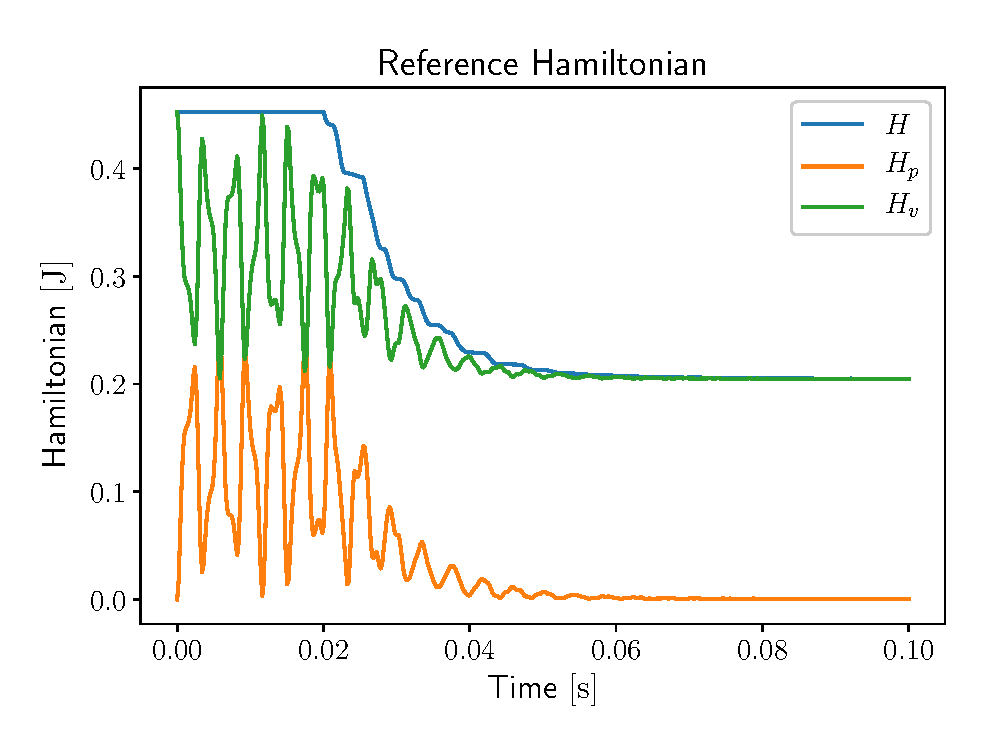
\includegraphics[width=0.48\columnwidth]{part_3/applications/mixed_bd_waves/Href.eps}}%
\hspace{8pt}%
\subfloat[][$L^2$ Hamiltonian error.]{%
\label{fig:Hdiff}%
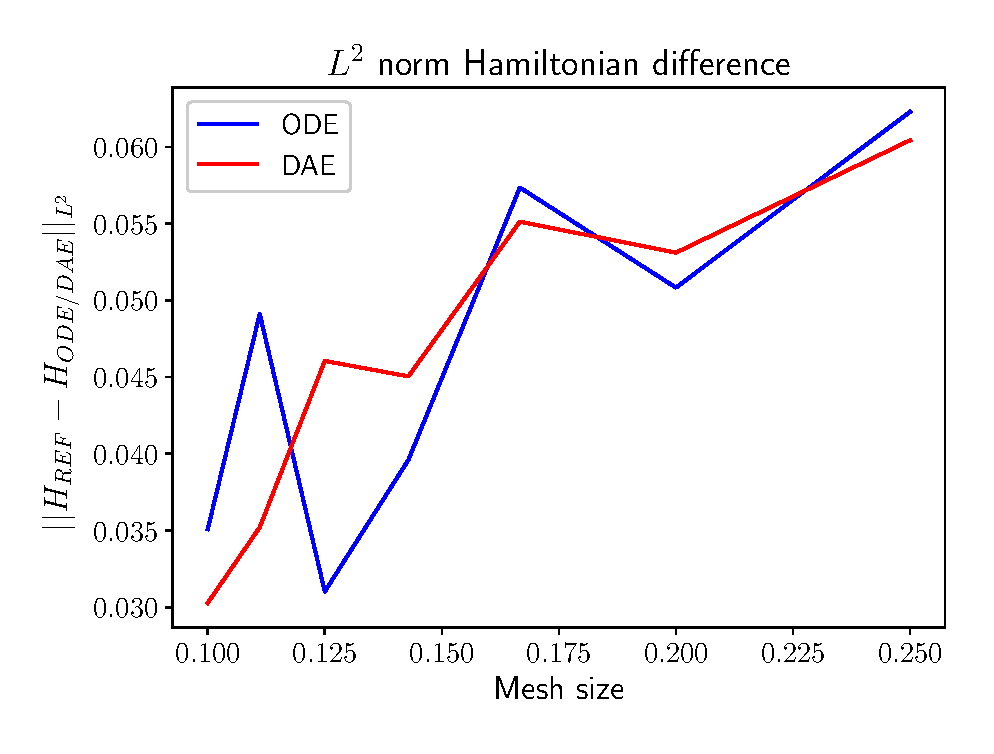
\includegraphics[width=0.48\columnwidth]{part_3/applications/mixed_bd_waves/Hall_diff.eps}} \\
\caption[]{Reference Hamiltonian and $L^2$ error.}%
\label{fig:Href_err}%
\end{figure}
}
\onslide*<3>{
\begin{figure}[ht]%
\centering
\subfloat[][$L^2$ pressure error.]{%
\label{fig:p_err}%
\includegraphics[width=0.48\columnwidth]{part_3/applications/mixed_bd_waves/err_ep.eps}}%
\hspace{8pt}%
\subfloat[][$L^2$ velocity error.]{%
\label{fig:v_err}%
\includegraphics[width=0.48\columnwidth]{part_3/applications/mixed_bd_waves/err_eq.eps}} \\
\caption[]{Error on the state variables for different mesh size.}%
\label{fig:error_x}%
\end{figure}
}

\begin{center}
	\onslide*<4>{
		\begin{columns}
			\begin{column}{.3\textwidth}
				\includemedia[
				label=vidNoRod,
				addresource=/home/a.brugnoli/Videos_defense/wave_dae15.mp4,
				activate=pageopen,
				width=4cm, height=5cm,
				flashvars={
					source=/home/a.brugnoli/Videos_defense/wave_dae15.mp4
					&loop=true
				}
				]{}{VPlayer.swf}
				Reference solution
			\end{column}		
			\begin{column}{.3\textwidth}
				\includemedia[
				label=vidNoRod,
				addresource=/home/a.brugnoli/Videos_defense/wave_dae10.mp4,
				activate=pageopen,
				width=4cm, height=5cm,
				flashvars={
					source=/home/a.brugnoli/Videos_defense/wave_dae10.mp4
					&loop=true
				}
				]{}{VPlayer.swf}
				DAE $h = L/10$
			\end{column}
			\begin{column}{.3\textwidth}
				\includemedia[
				label=vidRod,
				addresource=/home/a.brugnoli/Videos_defense/wave_ode10.mp4,
				activate=pageopen,
				width=4cm, height=5cm,
				flashvars={
					source=/home/a.brugnoli/Videos_defense/wave_ode10.mp4
					&loop=true
				}
				]{}{VPlayer.swf}
				ODE $h = L/10$
			\end{column}
		\end{columns}	
		\mediabutton[
		mediacommand=vidNoRod:playPause,
		mediacommand=vidRod:playPause
		]{\fbox{Play/Pause}}	
	}
\end{center}


\end{frame}


\section{PH flexible multibody dynamics}

\subsection{Detailed derivation of the equations of motion}

\begin{frame}{Equations of motion}
The equations are obtained by application of the virtual work principle \footfullcite[Chapter 4]{simeon2013computational}. \\
\begin{overlayarea}{\textwidth}{0.8\textheight}
	\only<1-3> {
		\begin{block}{Linear momentum balance}
			\setlength{\abovedisplayskip}{1pt}
			\setlength{\belowdisplayskip}{1pt}
			\only<1>{ 
				\begin{equation*}
				\begin{split}
				&m (\dot{\bm{v}}_P + \crmat{\bm{\omega}_P} \bm{v}_P) + \crmat{\bm{s}_u}^\top \dot{\bm{\omega}}_P  + \int_{\Omega} \rho \ddot{\bm{u}}_f \d{\Omega} = \\
				&\quad - \crmat{\bm{\omega}_P} \crmat{\bm{\omega}_P} \bm{s}_u - \int_{\Omega} 2 \rho \crmat{\bm{\omega}_P} \dot{\bm{u}}_f \d{\Omega} + \int_{\partial \Omega} \bm\tau \d{\Gamma},
				\end{split}
				\end{equation*}
			}
			\only<2>{
				\begin{equation*}
				\begin{split}
				m\dot{\bm{v}}_P + \crmat{\bm{s}_u}^\top \dot{\bm{\omega}}_P +   \int_{\Omega} \rho \dot{\bm{v}}_f \d{\Omega}  = \\
				\textcolor{red}{\left[m \bm{v}_P + \crmat{\bm{s}_u}^\top \bm\omega_P +2 \int_{\Omega} \rho \bm{v}_f \d{\Omega} \right]_\times} \bm\omega_P + \int_{\partial \Omega} \bm\tau \d{\Gamma}.
				\end{split}
				\end{equation*}
			}
			
			\only<3>{
				\begin{equation*}
				\begin{split}
				m\dot{\bm{v}}_P + \crmat{\bm{s}_u}^\top \dot{\bm{\omega}}_P +   \int_{\Omega} \rho \dot{\bm{v}}_f \d{\Omega}  = \textcolor{red}{\left[\widehat{\bm{p}}_t \right]_\times} \bm\omega_P + \int_{\partial \Omega} \bm\tau \d{\Gamma}.
				\end{split}
				\end{equation*}
			}
		\end{block}
		
	}
	
	\only<4-6> {
		\begin{block}{Angular momentum balance}
			\setlength{\abovedisplayskip}{1pt}
			\setlength{\belowdisplayskip}{1pt}
			\only<4>{
				\begin{equation*}
				\begin{split}
				\crmat{\bm{s}_u} (\dot{\bm{v}}_P + \crmat{\bm{\omega}_P} \bm{v}_P) + \bm{J}_u \dot{\bm\omega}_P + \int_{\Omega} \rho \crmat{\bm{x}+\bm{u}_f} \ddot{\bm{u}}_f \d{\Omega} + \crmat{\bm{\omega}_P} \bm{J}_u \bm{\omega}_P = \\ 
				- \int_{\Omega} 2\rho \crmat{\bm{x}+\bm{u}_f} \crmat{\bm\omega_P} \dot{\bm{u}}_f \d{\Omega} + \int_{\partial \Omega}\crmat{\bm{x}+\bm{u}_f} \bm\tau \d{\Gamma}, \\
				\end{split}
				\end{equation*}
			}
			\only<5>{
				\begin{equation*}
				\begin{split}
				\crmat{\bm{s}_u} \dot{\bm{v}}_P  + \bm{J}_u \dot{\bm\omega}_P + \int_{\Omega} \rho \crmat{\bm{x}+\bm{u}_f} \dot{\bm{v}}_f \d{\Omega} = \\
				\textcolor{red}{\left[\crmat{\bm{s}_u}^\top \bm\omega_P + 2 \int_{\Omega} \rho \bm{v}_f \d{\Omega} \right]_\times} \bm{v}_P +  \textcolor{red}{\left[\crmat{\bm{s}_u} \bm{v}_P + \bm{J}_u \bm\omega_P + 2 \int_{\Omega} \rho \crmat{\bm{x}+\bm{u}_f} {\bm{v}}_f \d{\Omega} \right]_\times} \bm\omega_P + 
				\\
				\int_{\Omega} \textcolor{red}{2 \left[\rho \bm{v}_P + \rho \crmat{\bm{x}+\bm{u}_f}^\top \, \bm\omega_P \right]_\times} \bm{v}_f \d{\Omega} + \int_{\partial \Omega}\crmat{\bm{x}+\bm{u}_f} \bm{\tau} \d{\Gamma}.
				\end{split}
				\end{equation*}
			}	
			
			\only<6>{
				\begin{equation*}
				\begin{split}
				\crmat{\bm{s}_u} \dot{\bm{v}}_P  + \bm{J}_u \dot{\bm\omega}_P + \int_{\Omega} \rho \crmat{\bm{x}+\bm{u}_f} \dot{\bm{v}}_f \d{\Omega} = \\
				\textcolor{red}{\left[\widehat{\bm{p}}_t \right]_\times} \bm{v}_P +  \textcolor{red}{\left[\widehat{\bm{p}}_r \right]_\times} \bm\omega_P + \textcolor{red}{\bm{\mathcal{I}}_{p_f}^{\Omega} } \bm{v}_f + \int_{\partial \Omega}\crmat{\bm{x}+\bm{u}_f} \bm{\tau} \d{\Gamma}.
				\end{split}
				\end{equation*}
			}	
		\end{block}
		
	}
	\only<7-9> {
		\begin{block}{Flexibility PDE}
			\setlength{\abovedisplayskip}{1pt}
			\setlength{\belowdisplayskip}{1pt}
			\only<7>{
				\begin{equation*}
				\begin{split}
				\rho (\dot{\bm{v}}_P + \crmat{\bm\omega_P} \bm{v}_P) + \rho (\crmat{\dot{\bm\omega}_P} + \crmat{\bm{\omega}_P}\crmat{\bm{\omega}_P})(\bm{x}+\bm{u}_f) + \rho (2 \crmat{\bm{\omega}_P} \dot{\bm{u}}_f + \ddot{\bm{u}}_f) = \Div{\bm\Sigma},
				\end{split}
				\end{equation*}
			}
			\only<8>{
				\begin{equation*}
				\begin{split}
				\rho \dot{\bm{v}}_P + \rho \crmat{\bm{x}+\bm{u}_f}^\top \dot{\bm\omega}_P  + \rho \dot{\bm{v}}_f = 
				\textcolor{red}{\left[\rho \bm{v}_P + \rho \crmat{\bm{x}+\bm{u}_f}^\top \bm\omega_P + 2 \rho \bm{v}_f \right]_\times} \bm\omega_P + \Div{\bm\Sigma}.
				\end{split}
				\end{equation*}
			}
			
			\only<9>{
				\begin{equation*}
				\begin{split}
				\rho \dot{\bm{v}}_P + \rho \crmat{\bm{x}+\bm{u}_f}^\top \dot{\bm\omega}_P  + \rho \dot{\bm{v}}_f = 
				\textcolor{red}{- \delta_{\bm{u}_f} H - \bm{\mathcal{I}}_{p_f}^*\bm\omega_P  }  + \Div{\bm\Sigma}.
				\end{split}
				\end{equation*}
			}
		\end{block}	
		
		together with boundary conditions
		\begin{equation*}
		\begin{aligned}
		&\text{Neumann condition} \\
		&\text{Dirichlet condition} \\
		\end{aligned} \quad
		\begin{aligned}
		\bm\Sigma \cdot \bm{n}|_{\Gamma_N} &= \bm\tau|_{\Gamma_N}, \quad \text{$\bm{n}$ is the outward normal,} \\
		\bm{u}_f|_{\Gamma_D} &= \bm{\bar{u}}_f|_{\Gamma_D},
		\end{aligned}
		\end{equation*}
	}
\end{overlayarea}
\end{frame}


\subsection{Construction of multibody chains: the example of planar beams}

\begin{frame}{Thin planar beam case}
\begin{columns}[T]
	\begin{column}{0.5\columnwidth}
		\begin{tcolorbox}
			\begin{figure}
				\centering
				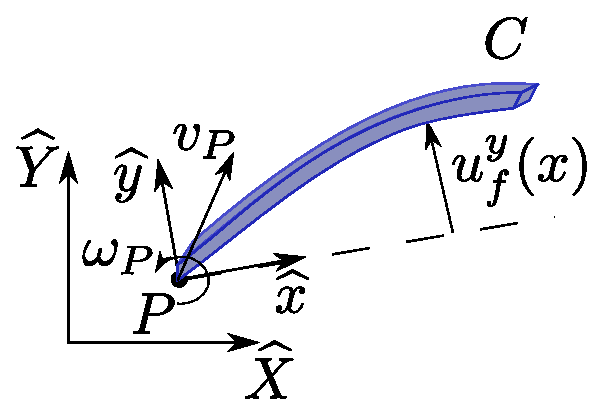
\includegraphics[width=0.98\columnwidth]{part_4/pHfmd/beam.eps} 
				\caption{Floating beam.}
				\label{fig:beam}
			\end{figure}
		\end{tcolorbox}
	\end{column}
	\begin{column}{0.5\textwidth}
		\begin{block}{Beam discretized system}
			Neglecting the dependence on the deformation field in the mass matrix ($\mathbf{M}=\text{const}$)
			\begin{equation*}
			\begin{aligned}
			\mathbf{E} \dot{\mathbf{e}} &= \mathbf{J}(\mathbf{e}) \mathbf{z}(\mathbf{e}) + \mathbf{B} \mathbf{u}, \vspace{2mm} \\
			\mathbf{y} &= \mathbf{B}^{\top}  \mathbf{z}, \\
			\end{aligned}
			\end{equation*}
			with boundary variables
			\begin{equation*}
			\begin{aligned}
			\mathbf{u} &=  [F_{P}^x, \; F_{P}^y, \; T_{P}^z, \; F_{C}^x, \; F_{C}^y, \; T_{C}^z]^\top, \\
			\mathbf{y} &=  [v_{P}^x, \; v_{P}^y, \; \omega_{P}^z, \; v_{C}^x, \; v_{C}^y, \; \omega_{C}^z]^\top.
			\end{aligned}
			\end{equation*}
		\end{block}	
	\end{column}
\end{columns}

\end{frame}

\begin{frame}{Revolute joint between beams}
\begin{columns}
\begin{column}{0.5\textwidth}
	\begin{tcolorbox}
		\begin{figure}[t]
			\centering
			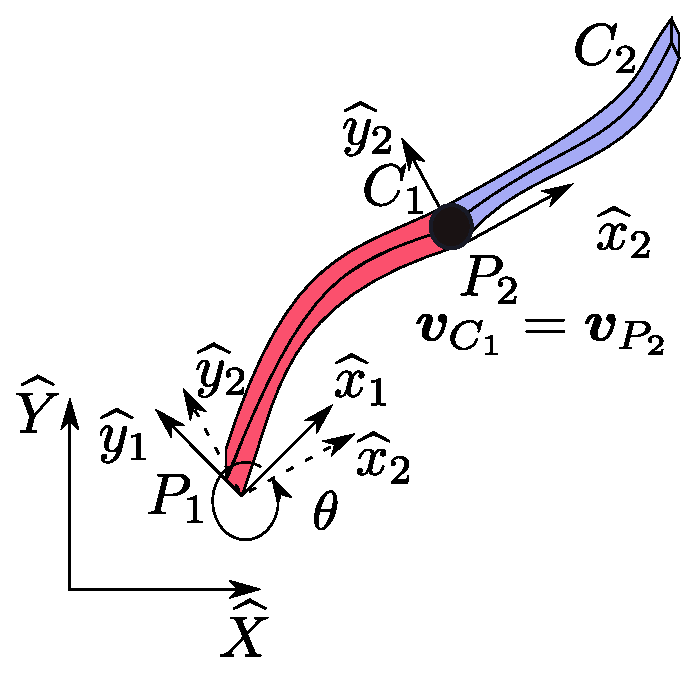
\includegraphics[width=0.9\columnwidth]{part_4/pHfmd/beam_int.eps} 
			\caption{Two hinged beams.}
			\label{fig:beam_int}
		\end{figure}
	\end{tcolorbox}
\end{column}
\begin{column}{0.5\textwidth}
	The interconnection variables are
	\begin{equation*}
	\begin{aligned}
	\mathbf{u}_1^{\text{int}} &= [F^x_{C_1}, \, F^y_{C_1}]^\top := \mathbf{F}_{C_1}, \\
	\mathbf{u}_2^{\text{int}} &= [F^x_{P_2}, \, F^y_{P_2}]^\top := \mathbf{F}_{P_2}, \\
	\mathbf{y}_1^{\text{int}} &= [v^x_{C_1}, \, v^y_{C_1}]^\top := \mathbf{v}_{C_1}, \\
	\mathbf{y}_2^{\text{int}} &= [v^x_{P_2}, \, v^y_{P_2}]^\top := \mathbf{v}_{P_2}.
	\end{aligned}
	\end{equation*}
	
\end{column}
\end{columns}

\end{frame}

\begin{frame}{Final system}
\begin{block}{Hinged interconnected beams}
The transformer interconnection
\begin{equation*}
\mathbf{u}_1^{\text{int}} = -\mathbf{R}(\theta) \mathbf{u}_2^{\text{int}}, \qquad
\mathbf{y}_2^{\text{int}} = \mathbf{R}(\theta)^\top \mathbf{y}_1^{\text{int}},
\end{equation*}
where $\mathbf{R}(\theta)$ is the relative rotation matrix,	imposes the constraints on the velocity level and gives rise to a quasi-linear index 2 pHDAE.
\begin{equation*}
\begin{aligned}
\begin{bmatrix}
\mathbf{E}_1 & 0 & 0 \\ 
0 & \mathbf{E}_2 & 0 \\
0 & 0 & 0 \\
\end{bmatrix}
\begin{bmatrix}
\dot{\mathbf{e}}_1 \\ \dot{\mathbf{e}}_2 \\ \dot{\bm{\lambda}} \\
\end{bmatrix} &= 
\begin{bmatrix}
\mathbf{J}_1(\mathbf{e}_1) & 0 & -\mathbf{B}_1^{\text{int}} \mathbf{R} \\ 
0 & \mathbf{J}_2(\mathbf{e}_2) & \mathbf{B}_2^{\text{int}} \\
\mathbf{R}^\top \mathbf{B}_1^{\text{int} \top} & - \mathbf{B}_2^{\text{int} \top} & 0 \\
\end{bmatrix}
\begin{bmatrix}
\mathbf{z}_1  \\ 
\mathbf{z}_2  \\ 
\bm{\lambda} \\
\end{bmatrix}+ 
\begin{bmatrix}
\mathbf{B}_{\partial 1}^{\text{ext}} & 0 \\ 0 & \mathbf{B}_{\partial 2}^{\text{ext}} \\ 0 & 0 \\
\end{bmatrix} 
\begin{bmatrix}
\mathbf{u}_1^{\text{ext}} \\ 
\mathbf{u}_2^{\text{ext}} \\
\end{bmatrix}, \\
\begin{bmatrix}
\mathbf{y}_1^{\text{ext}} \\ \mathbf{y}_2^{\text{ext}} \\
\end{bmatrix}  &= \begin{bmatrix}
\mathbf{B}_{\partial 1}^{\text{ext} \top} & 0 & 0 \\
0 & \mathbf{B}_{\partial 2}^{\text{ext} \top} & 0 \\
\end{bmatrix} \begin{bmatrix}
\mathbf{z}_1  \\ 
\mathbf{z}_2  \\ 
\bm{\lambda} \\
\end{bmatrix}.
\end{aligned}
\end{equation*}
\end{block}
\end{frame}

\subsection{Details on the Kirchhoff plate interconnection}

\begin{frame}{Boundary interconnection}
\only<1>{
	The system is composed by a cantilever plate (distributed pH) connected to a rigid rod:
	\begin{minipage}{.45\linewidth}
		\begin{equation*}
		\text{dpH}\qquad
		\begin{aligned}
		\partial_t \bm{x}_1 &= \mathcal{J} \, \delta_{\bm{x}_1} {H_1}, \\
		\bm{u}_{\partial, 1}  &= \mathcal{B}_\partial \, \delta_{\bm{x}_1} {H_1}, \\
		\bm{y}_{\partial, 1} &= \mathcal{C}_\partial \, \delta_{\bm{x}_1} {H_1}, \\
		\end{aligned}
		\end{equation*}
	\end{minipage}
	\begin{minipage}{.5\linewidth}
		\begin{equation*}
		\text{pH} \qquad
		\begin{aligned}
		\dot{\mathbf{x}}_2 &= \mathbf{J} \nabla_{\mathbf{x}_2} {H_2} + \mathbf{B} \mathbf{u}_2, \\
		\mathbf{y}_{2} &= \mathbf{B}^\top \nabla_{\mathbf{x}_2} {H_2}, \\
		\end{aligned}
		\end{equation*}
	\end{minipage} %
	
	\vspace{.3cm}
	
	where $\mathbf{x} \in \mathbb{R}^n, \mathbf{u}_2, \mathbf{y}_2 \in \mathbb{R}^m$ and $\bm{x}_1 \in {X}$,  $\bm{u}_{\partial, 1}  \in {U}, \, \bm{y}_{\partial, 1} \in  {Y} = {U}^\prime$ belong to and Hilbert spaces  and  $\mathcal{B}_\partial: {X} \rightarrow {U}, \; \mathcal{C}_\partial: {X} \rightarrow {Y}$ are boundary operators. \\ The duality pairings for the boundary ports are denoted by
	\[
	\inner[{U} \times {Y}]{\bm{u}_{\partial, 1}}{\bm{y}_{\partial, 1}},  \qquad
	\inner[\mathbb{R}^m]{\mathbf{u}_{2}}{\mathbf{y}_{2}}.
	\]
	For the interconnection, consider the compact operator $\mathcal{W}: Y \rightarrow \mathbb{R}^m$ and the following power-preserving interconnection
	\begin{equation*}
	\label{eq:int_inf}
	\mathbf{u}_2 = -\mathcal{W} \, \bm{y}_{\partial, 1},  \qquad \bm{u}_{\partial, 1} = \mathcal{W}^* \, \mathbf{y}_2.
	\end{equation*}
}

\only<2>{\vspace{.5cm}\centering \includegraphics[width=0.6\textwidth]{part_4/validation/KP/pp_interconnection.eps}}

\end{frame}

\begin{frame}{Kirchhoff plate welded to a rigid rod}
\begin{equation*}\small
\begin{aligned}
\text{Plate} \; (\Omega &= [0, L_x] \times [0, L_y]) \\
\begin{bmatrix}
\rho h & 0 \\ 0 & \mathcal{\bm{C}}_b \\
\end{bmatrix}
\diffp{}{t}
\begin{bmatrix}
{e}_w \\ \bm{E}_\kappa \\
\end{bmatrix} &= 
\begin{bmatrix}
0 & -\div\Div \\ \nabla^2 & 0 \\
\end{bmatrix}
\begin{bmatrix}
{e}_w \\ \bm{E}_\kappa \\
\end{bmatrix} \\
u_{\partial, \text{pl}} &= {e}_w (x = L_x, y), \\
y_{\partial, \text{pl}} &= \widetilde{q}_n(x = L_x, y).
\end{aligned} \qquad \quad
\begin{aligned}
\text{Rigid rod} \\
\begin{bmatrix}
M & 0 \\
0   & J_G \\
\end{bmatrix} 
\displaystyle \diff{}{t}
\begin{pmatrix}
v_G \\ \omega_G \\
\end{pmatrix} & = \begin{pmatrix}
F_z \\ T_x \\
\end{pmatrix} = \bm{u}_{\text{rod}}\vspace{1mm}, \\
\bm{y}_{\text{rod}} &= \begin{pmatrix}
v_G \\ \omega_{G} \\
\end{pmatrix},
\end{aligned}
\end{equation*}
Space $Y$ is the space of square-integrable functions with support on $\Gamma_{\text{int}} = \left\{x=L_x\right\}$. \\
The interconnection operator  provides the total force and torque acting on the rigid rod
\begin{equation*}
\mathcal{W} y_{\partial, \text{pl}} =  - \begin{pmatrix}
F_z \\
T_x \\
\end{pmatrix} = \begin{pmatrix}
\int_{\Gamma_{\text{int}}} y_{\partial, \text{pl}} \d{s} \\
\int_{\Gamma_{\text{int}}} \left( y - L_y/2 \right) y_{\partial, \text{pl}} \d{s} \\
\end{pmatrix}.
\end{equation*}
The adjoint operator provides a rigid movement as the plate input at $\Gamma_{\text{int}}$
\begin{align*}
\left\langle \mathcal{W} y_{\partial, \text{pl}}, \; \bm{y}_{\text{rod}} \right\rangle_{\mathbb{R}^m} &= \left\langle y_{\partial, \text{pl}}, \, \mathcal{W}^* \bm{y}_{\text{rod}}\right\rangle_{L^2(\Gamma_{\text{int}})}, \\
\mathcal{W}^* {y}_{\text{rod}} &= v_G + \omega_{G} \left( y - L_y/2 \right).
\end{align*}
\end{frame}


\end{document}
